%!TEX root =  ../main.tex

\mychapters{Polynomials}{polynomials}{\chapdir/pics/Sao_Paulo_Stock_Exchange.jpg}

Polynomials are among the most well-studied and understood parts of mathematics.
There is a tremendous amount we know and can describe about how they work
and what parts of the natural world they describe.  However, this is still so much
to discover about them and it is readily possible to generate unsolvable problems.

That being said, monstrously difficult problems become easily doable with the mastery
of a few, simple techniques.  Does this look easy?!


\begin{equation}
135x^{10} + 54x^9 + 5x^7 + 2x^6 - 135x^4 - 54x^3 - 5x - 2 = 0
\end{equation}

You might not believe it, but if we told you $-\frac{2}{5}$ was one of the solutions, 
the rest will jump out at you in no time flat!


\newpage
\chapterminitoc


%									6 - 1
\newpage
\invisiblesection{Graphs}
\marginlessinput{\chapdir/0601p}
\newpage
%!TEX root =  ../main.tex

\subsection{Definition}

\objective{Describe and predict the general shape of a polynomial graph}


A polynomials is sum of terms, all of which are of the form $a\cdot{}x^n$, where $a$
is any rational number and $n$ is a whole number.

\subsubsection{Degree}
``In the long run, the biggest exponent always wins.''  While it may sound like a odd
cliche from a movie, it is certainly true.  What is more, there are only two possibilities
for polynomials: either larger and larger numbers are being raised to an even degree,
or they are being raised to an odd one.  Positive numbers grow more positive in either case.
Negative numbers become positive, when raised to an even degree.  They grow more
negative when raised to an odd degree.

Of course, in the short, all manner of other behaviors may be manifested, but it is 
important to consider limits at the infinities, so that we may be sure of the ultimate
leftward or rightward behavior of a function.

\subsubsection{Leading Coefficient}
While it is true that there are only two possibilities for the integer $n$ in the 
expression $x^n$ (either it is even, or it is odd), there are two more things that could 
happen, when we consider $a\cdot{}x^n$: $a$ could be positive or negative.
In summary, even polynomials go ``up'' at both ``ends'', unless the leading coefficient
is negative, in which case both ends go ``down''.  Odd functions go up to the right and
down to the left, unless the leading coefficient is negative, in which case the opposite
happens.

If we are designing a function ourselves, it can still be useful to consider
end-run behavior.  For example, we might construct a polynomial to have
$x$-intercepts 3, 5, and $-\frac{1}{2}$.  We would write $f(x)=(x-3)(x-5)(2x+1)$,
seemingly obfuscating the leading term.  However, if we multiply only the $x$ terms,
we can still find it quickly.  $x \cdot x \cdot 2x$ is $2x^3$, so we can see this is
a positive, odd polynomial, going up to the right and down to the left.

\subsubsection{$y$-intercept}
Another facet of polynomials that is still quickly discernible even in factored form
is the constant term.  This term (even if it is 0, i.e. absent) provides useful information.
When $x=0$ (which typically corresponds to something like an initial condition), the
only term not to cancel will be the constant one.  In the previous example, we can 
easily multiply the plain numbers: $-3 \cdot -5 \cdot 1 = 15$, so we know the
$y$-intercept of the function will be 15.  If we need a different number, the function
can always be scaled by multiplying on the outside by a constant, which could even
be negative.

\subsection{Factored Forms}
When we examined quadratics, there were some cases in which the vertex of the
parabola was found on the $x$-axis.  A similar case can be found in polynomials of
higher degree, and can be seen in their factored forms.  For example,
$f(x)= (x-2)^2(x+5)$ is a cubic equation  (with leading term $x^3$ and constant term
20) which seems to have only two zero's: 2 and -5.  However, the number 2 works as
a solution \emph{twice}, and so we say it has a \textbf{multiplicity} of 2.

Graphically, multiplicity means the graph resembles the exponent of the factored term.
This means $f(x)$ will behave like $x^2$ in the vicinity of 2.  Note that this behavior
may be upside-down, depending on the equation.  Generalizing even more, we can say
that even powers on a factor will result in the graph \emph{not} crossing the $x$-axis
at that zero, but only ``bouncing'' off.  On the other hand, odd powers on a factor
(even including 1!) will appear as the graph proceeding \emph{through} the $x$-axis.


\newpage
\subsection{Exercises}
Kuta



%									6 - 2
\newpage
\section{Factoring}
\noindent\makebox[\textwidth]{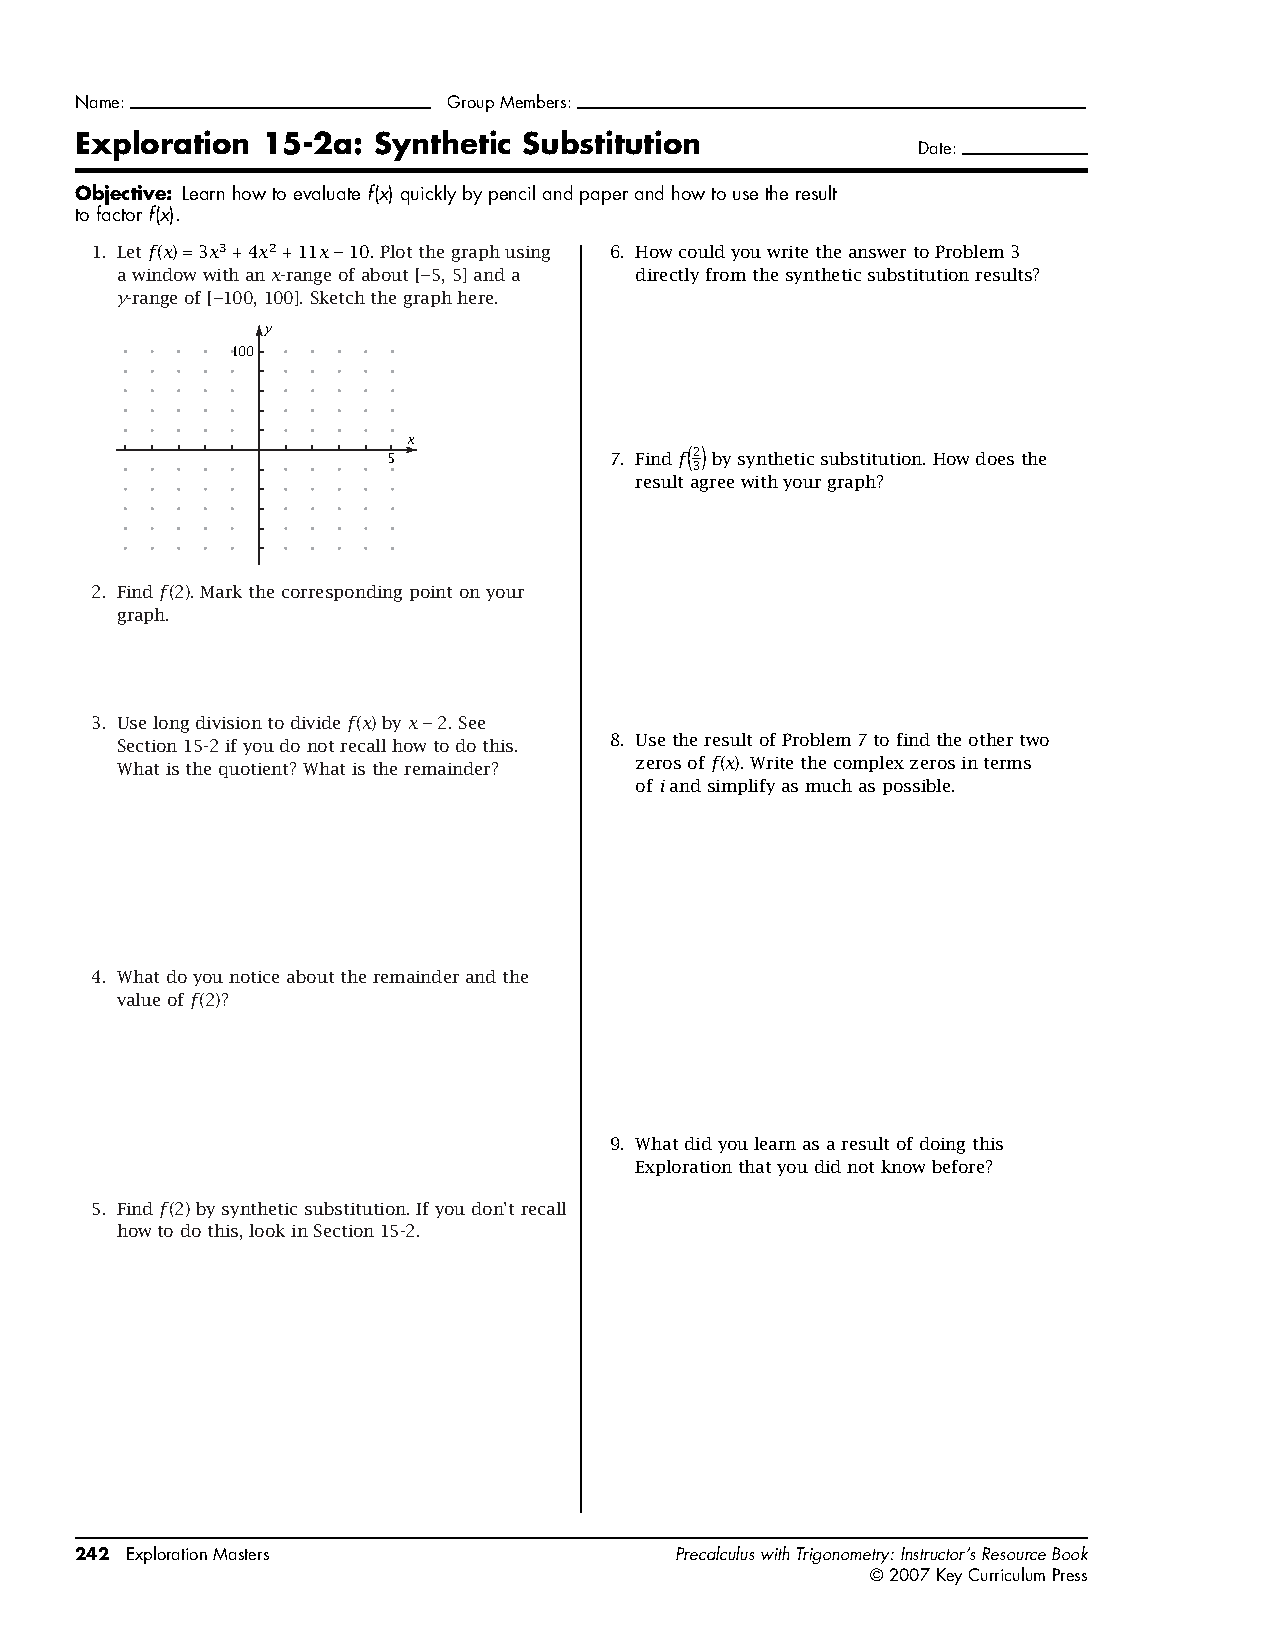
\includegraphics[width=\paperwidth]{\chapdir/0602p.pdf}}
%!TEX root =  ../main.tex

\subsection{Polynomial Long Division}

\objective{Use and known when to use polynomial and synthetic division}


First, we recall long division.  Surprisingly, it can actually be more difficult than polynomial long division at times, so we should pick an easy example:

\vspace{5mm}

\longdiv{11}{3678}

We restrict our vision to the left two digits of the dividend, as we know that 11 will go 3 times into
36.  We write a 3 above the 6, write 33 below the 36 and subtract it.  Next, we bring down the 7
and do the same manner of work on 37.  The process repeats, but moves progressively right
and we get an answer of 334, but with a remainder of 4.  Since we most want a number that
when multiplied by 11 obtains 3678, we should write the answer as $334+\frac{4}{11}$ because
$\left(334+\frac{4}{11}\right)(11) = 3678$.


Now, polynomial long division is no different.  We start at the left edge of the dividend, and use 
only the leading term of the divisor.

\polylongdiv[stage=3]{x^3-x^2+x-1}{x+1}

We only regarded the leading (left) edge of the larger polynomial.  In this case, that is $x^3$.  
We might ask ourselves, ``What do I need to multiply $x$ by to get to $x^3$?''.  The answer is $x^2$.  
That term is the first in our quotient, and we multiply it by the entire divisor.  We subtract, 
and bring down the next term.

\polylongdiv[stage=4]{x^3-x^2+x-1}{x+1}

This process continues, only working on the left-edge as we go down.  

\polylongdiv[stage=13]{x^3-x^2+x-1}{x+1}

The final answer is $x^3-x^2+x-1 = (x+1)\left(x^2-2x+3-\cfrac{4}{x+1}\right)$.

\subsection{Synthetic Division}
One might ask, ``Isn't there a faster way?'' and indeed there is.  Let us first consider
how we might compactify the polynomial.  Consider the first two terms, and look for
a common factor:
$$
(x^3-x^2)+x-1
$$
Obviously, we can take out an $x^2$ from the first two terms.  Having condensed the
first two terms into one (because multiplication does not increase the term count),
now consider the greatest common factor of the new first two term:
$$
\left[x^2(x-1)+x\right]-1
$$
Every term has at least one $x$, so that can be safely factored out.  Look at what we have made,
called \textbf{nested form}:
$$
x\left[(x-1)x+1\right]-1
$$
Substituting any value into this function now only involves multiplication and addition/subtraction,
ever exponents.  This process can be represented in half-box, called \textbf{synthetic division}

\polyhornerscheme[showvar=true,resultbottomrule=true,resultleftrule=true,resultrightrule=true,x=-1]{x^3-x^2+x-1}

Study this carefully, and notice how it is the same answer as the coefficients of the polynomial
long division problem.  There are lots of things to notice.  The technique with synthetic division is
to remember that the first number falls straight down, but from then on we  ``multiply up, add down''.  
It is helpful to draw a box around the final number, to remember that it is special: it is the remainder.  
Reading right-to-left: 3 is the $x^0$ coefficient, $-2$ is on $x^1$, 1 is on $x^2$.  
In the long division, we divided by $x + 1$.  Here, we are plugging in a value, so it's $x + 1 = 0$, 
which is $x=-1$. 

\begin{example}[Synthetic Division]
Given $g(x) = x^3-7x+6$, find $g(2)$.  What does this tell you about $\frac{g(x)}{x-2}$?

\paragraph{Solution}
First, we write our box and the $x=$ we want to test:\\


\polyhornerscheme[showvar=true,stage=1,x=2]{x^3-7x+6}
(Note the zero.  Failure to notice this is crucial mistake!)


The first number passes down freely:
\polyhornerscheme[showvar=true,tutor=true,stage=2,x=2]{x^3-7x+6}


Then we ``multiply up...
\polyhornerscheme[showvar=true,tutor=true,stage=3,x=2]{x^3-7x+6}


..., add down''
\polyhornerscheme[showvar=true,tutor=true,stage=4,x=2]{x^3-7x+6}


and so on and so forth:
\polyhornerscheme[showvar=true,resultbottomrule=true,resultleftrule=true,resultrightrule=true,x=2]{x^3-7x+6}

The fact that the remainder is 0 is significant.  $(x-2)$ is a factor in $x^3-7x+6$.  We can write
this as $(x-2)(x^2+2x-3)=x^3-7x+6$.  The quadratic factors easily into (x+3)(x-1), leaving the
entire cubic equation solved.
\end{example}

\subsection{Complex Zeros}
What if nothing so need exists as a solution?  We might slightly alter our $g(x)$ to be
$x^3-2x^2-7x+2$.  There is no easy factorization (grouping won't work).  We are forced
to use more complicated algorithms.  In the past, mathematicians invented very complicated
methods for find, eliminating, and testing solutions to polynomial equations.  You will research
one of these in problem number one of the exercises.  But in our age, why not use a computer?
If done intelligently, we can get the same level of precision as in the past.

For example, if you take our new $g(x)$ and put it in your TI-8*, you can see --- either in the
TABLE or on the graph --- that it passes through (-3,0), which should lead you to want to
factor out (x+3).  You can use synthetic division as so:


\polyhornerscheme[showvar=true,resultbottomrule=true,resultleftrule=true,resultrightrule=true,x=-3]{x^3-2x^2-7x+24}

This proves that $(x+3)(x^2-5x+8)=x^3-2x^2-7x+24$.  However, now we have a new problem: how
can we solve $x^2-5x+8=0$?  It is not factorable.  Well, any quadratic can be solved with
the quadratic formula, so that will have to do.

$$
x=\frac{5\pm\sqrt{(-5)^2-4(1)(8)}}{2\cdot{}1}
=\frac{5\pm i\sqrt{7}}{2}
$$

As you can see, unfactorable quadratics will always have some quantity inside the square root,
once plugged into the quadratic formula.  This means they will produce either a pair of
irrational solutions, or else a pair of complex (imaginary) ones.  This has other to prove
(elsewhere) that such solutions \emph{always} occur in pairs.

For example, if we are building a polynomial, and we know solutions include 2 and $3+2i$,
then we can be sure that $3-2i$ is also a solution.  What factor would produce such zeros?
Well, x-2 is an obvious one, but what about the more difficult one?  If $x=3 \pm 2i$, what
would have lead to two possibilities like that?

\begin{align*}
  x & = 3 \pm 2i\\
  x - 3 & =  2i \\
  (x-3)^2 & = -5\\
  x^2-6x+9 &= -5\\
  x^2-6x+14 &= 0
\end{align*}

Since plus-or-minus solution come from square rooting, the inverse operation must be to
square both sides.  $(+2i)(+2i) = (-2i)(-2i) = -5$, so writing plus or minus does not matter.

\newpage
\subsection{Exercises}
In Kuta



%									6 - 3
\newpage
\invisiblesection{Mean, Max., Min.}
\marginlessinput{\chapdir/0603p}
\newpage
%!TEX root =  ../main.tex

\objective{Use derivative and integrals to calculate mean, max, and min}

\subsection{Extrema}
Most often, real-life models of continuously changing outputs (which graph as curved lines)
are useful to find maximums and minimum.  Zeros are important --- all the more so when
they appear in the denominator --- but extrema are typically more.  (Extrema is collective
term for both maximum and minimums.)  Calculus is extremely useful in finding these moments.

\index{derivative!test}
This about the some continuous, smooth curve.  What is the derivative measuring?  It is the
slope of the function at every point.  If it is positive, the function is increasing.  If it is
negative, the function is decreasing.  If it is constant, the function is level.  Even if this happens
only for an instant, it is noteworthy.  But there are three things which might be happening
\begin{enumerate}
\item the function might have been decreasing and is switching to increasing
\item the function might have been increasing and is switching to decreasing
\item the function may be pausing in its ascend or descend, but will resume forthwith
\end{enumerate}

Consider $x^3$ vs. $x^2$.  Both functions have a derivative of 0 at $x=0$.  Only one has
an extremity, while the other has a saddle point.  The key to telling the difference numerically
is to see what the rate of change of the rate of change is doing, i.e. the second derivative.
Just as the first derivative tells us about the slope of a function, the second derivative tells us about
concavity or convexity.  A concave region of a smooth, continuous function will have a minimum,
while a convex region will have a maximum.  So, unless we know the shape beforehand,
it is necessary to determine the second derivative too --- not just the first --- in order to know
where the extrema are.

\personfeature[-3in]{\chapdir/pics/GodfreyKneller-IsaacNewton-1689}{Isaac Newton}{1642-1726}{
was an English mathematician, astronomer, and physicist who is widely recognized as 
one of the most influential scientists of all time and a key figure in the scientific revolution.
The second fundamental theorem of calculus is also called the Newton–Leibniz axiom.
\href{https://en.wikipedia.org/wiki/Isaac_Newton}{Wikipedia}}

\subsection{Average Value}
The anti-derivative of a function tells us the area under the curve.  When done over an open
interval (called a definite integral) this has a remarkable side effect: it also tells us the average
value of function, no matter how curvy.  Normally we think of averages as adding up a finite set 
of values, and dividing by the number of quantities just added.  Strangely, this intuition works,
even over an infinite number of heights.

Consider the function $f(x)=-12(x^3-2x^2-11x+12)$.  If we are interested in the extrema, they 
occur when the derivative is 0.  The derivative is $-36x^2-48x-11$, which requires the Q.F. to
solve.  It's zeros are $\frac{2\pm\sqrt{37}}{3}$, or approximate .  The heights of the function
are $\frac{8}{9}(37\sqrt{37}\mp55)$ respectively.  But what about the area between each 
``hump'' and the $x$-axis?  For that we need the integral, which is $-3x^4+8x^3+66x^2+144x+C$.
Plugging in the zero, we find that $\int_1^4 f(x) = 297$ and $\int_{-3}^1 f(x) = -640$.

If we look at this right area, we see that we know its minimum height, it's maximum height, and
it's area.  There must exist some average height of the function, because we can imagine a rectangle
with a base of 3 and that height, which has an area of 297.  By simple division, that height must be
99.  The average value of the continuous curve $f(x)$ from 1 to 4, is 99.


\begin{figure}[h]
\begin{centering}
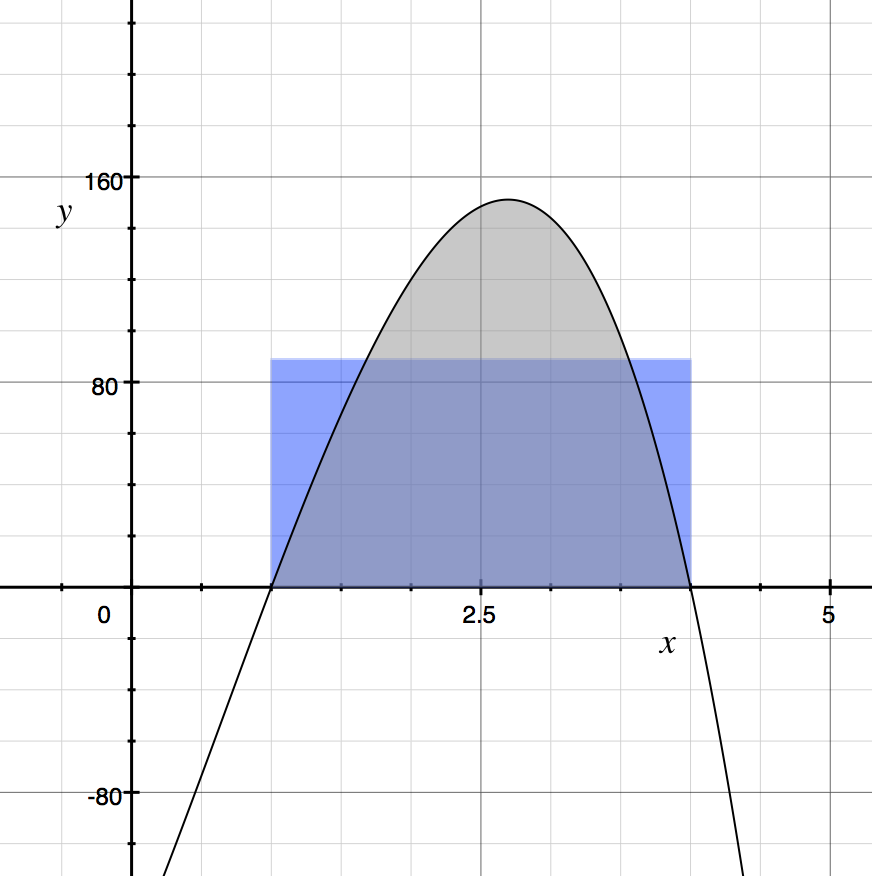
\includegraphics[scale=0.5]{\chapdir/pics/averageintegral}\index{integral!to the average}
\caption[Integrals and Averages]{A rectangle with height at the function's average value has the same area as the integral over the same width.}
\end{centering}
\end{figure}

How can this be?  Imagine if we cut the region up into finitely many pieces.  The average height
is equal to the sum of the heights at every point in our sample group, divided by the number of
samples, $n$, that we have cut the width up into.  
In this case, let us write this sum using the integral sign.

$$
\cfrac{\text{The sum of the heights of} f(x) \text{every} \frac{4-1}{n}}{\frac{4-1}{n}}
$$

But we really ought to use the integral sign, because we don't actually want to cut up the region into
a finite number ($n$) of slices, but an infinite number, with each step being no more than $dx$ wide.
This means we should've written

$$
\cfrac{\int_1^4 f(x)}{\frac{4-1}{dx}} = \frac{\int_1^4 f(x)dx}{4-1}
$$

Because dividing twice is the same as multiplying, our infinitely many additions in the numerator
has suddenly because an infinite number of areas, with infinitely many rectangles being brought
together and summed up --- integrated, each one the height of the function times the infinitely
narrow width $dx$.  In other words, the definite integral over a region, divided by the width of
the region equals the average height of the region.

$$
\frac{\int_a^b f(x)}{b-a} = \frac{F(b)-F(a)}{b-a} = \text{average height}
$$

This is also known as the Fundamental Theorem of Calculus.\index{Fundamental Theorem of Calculus}
\newpage
\subsection{Exercises}
\noindent\makebox[\textwidth]{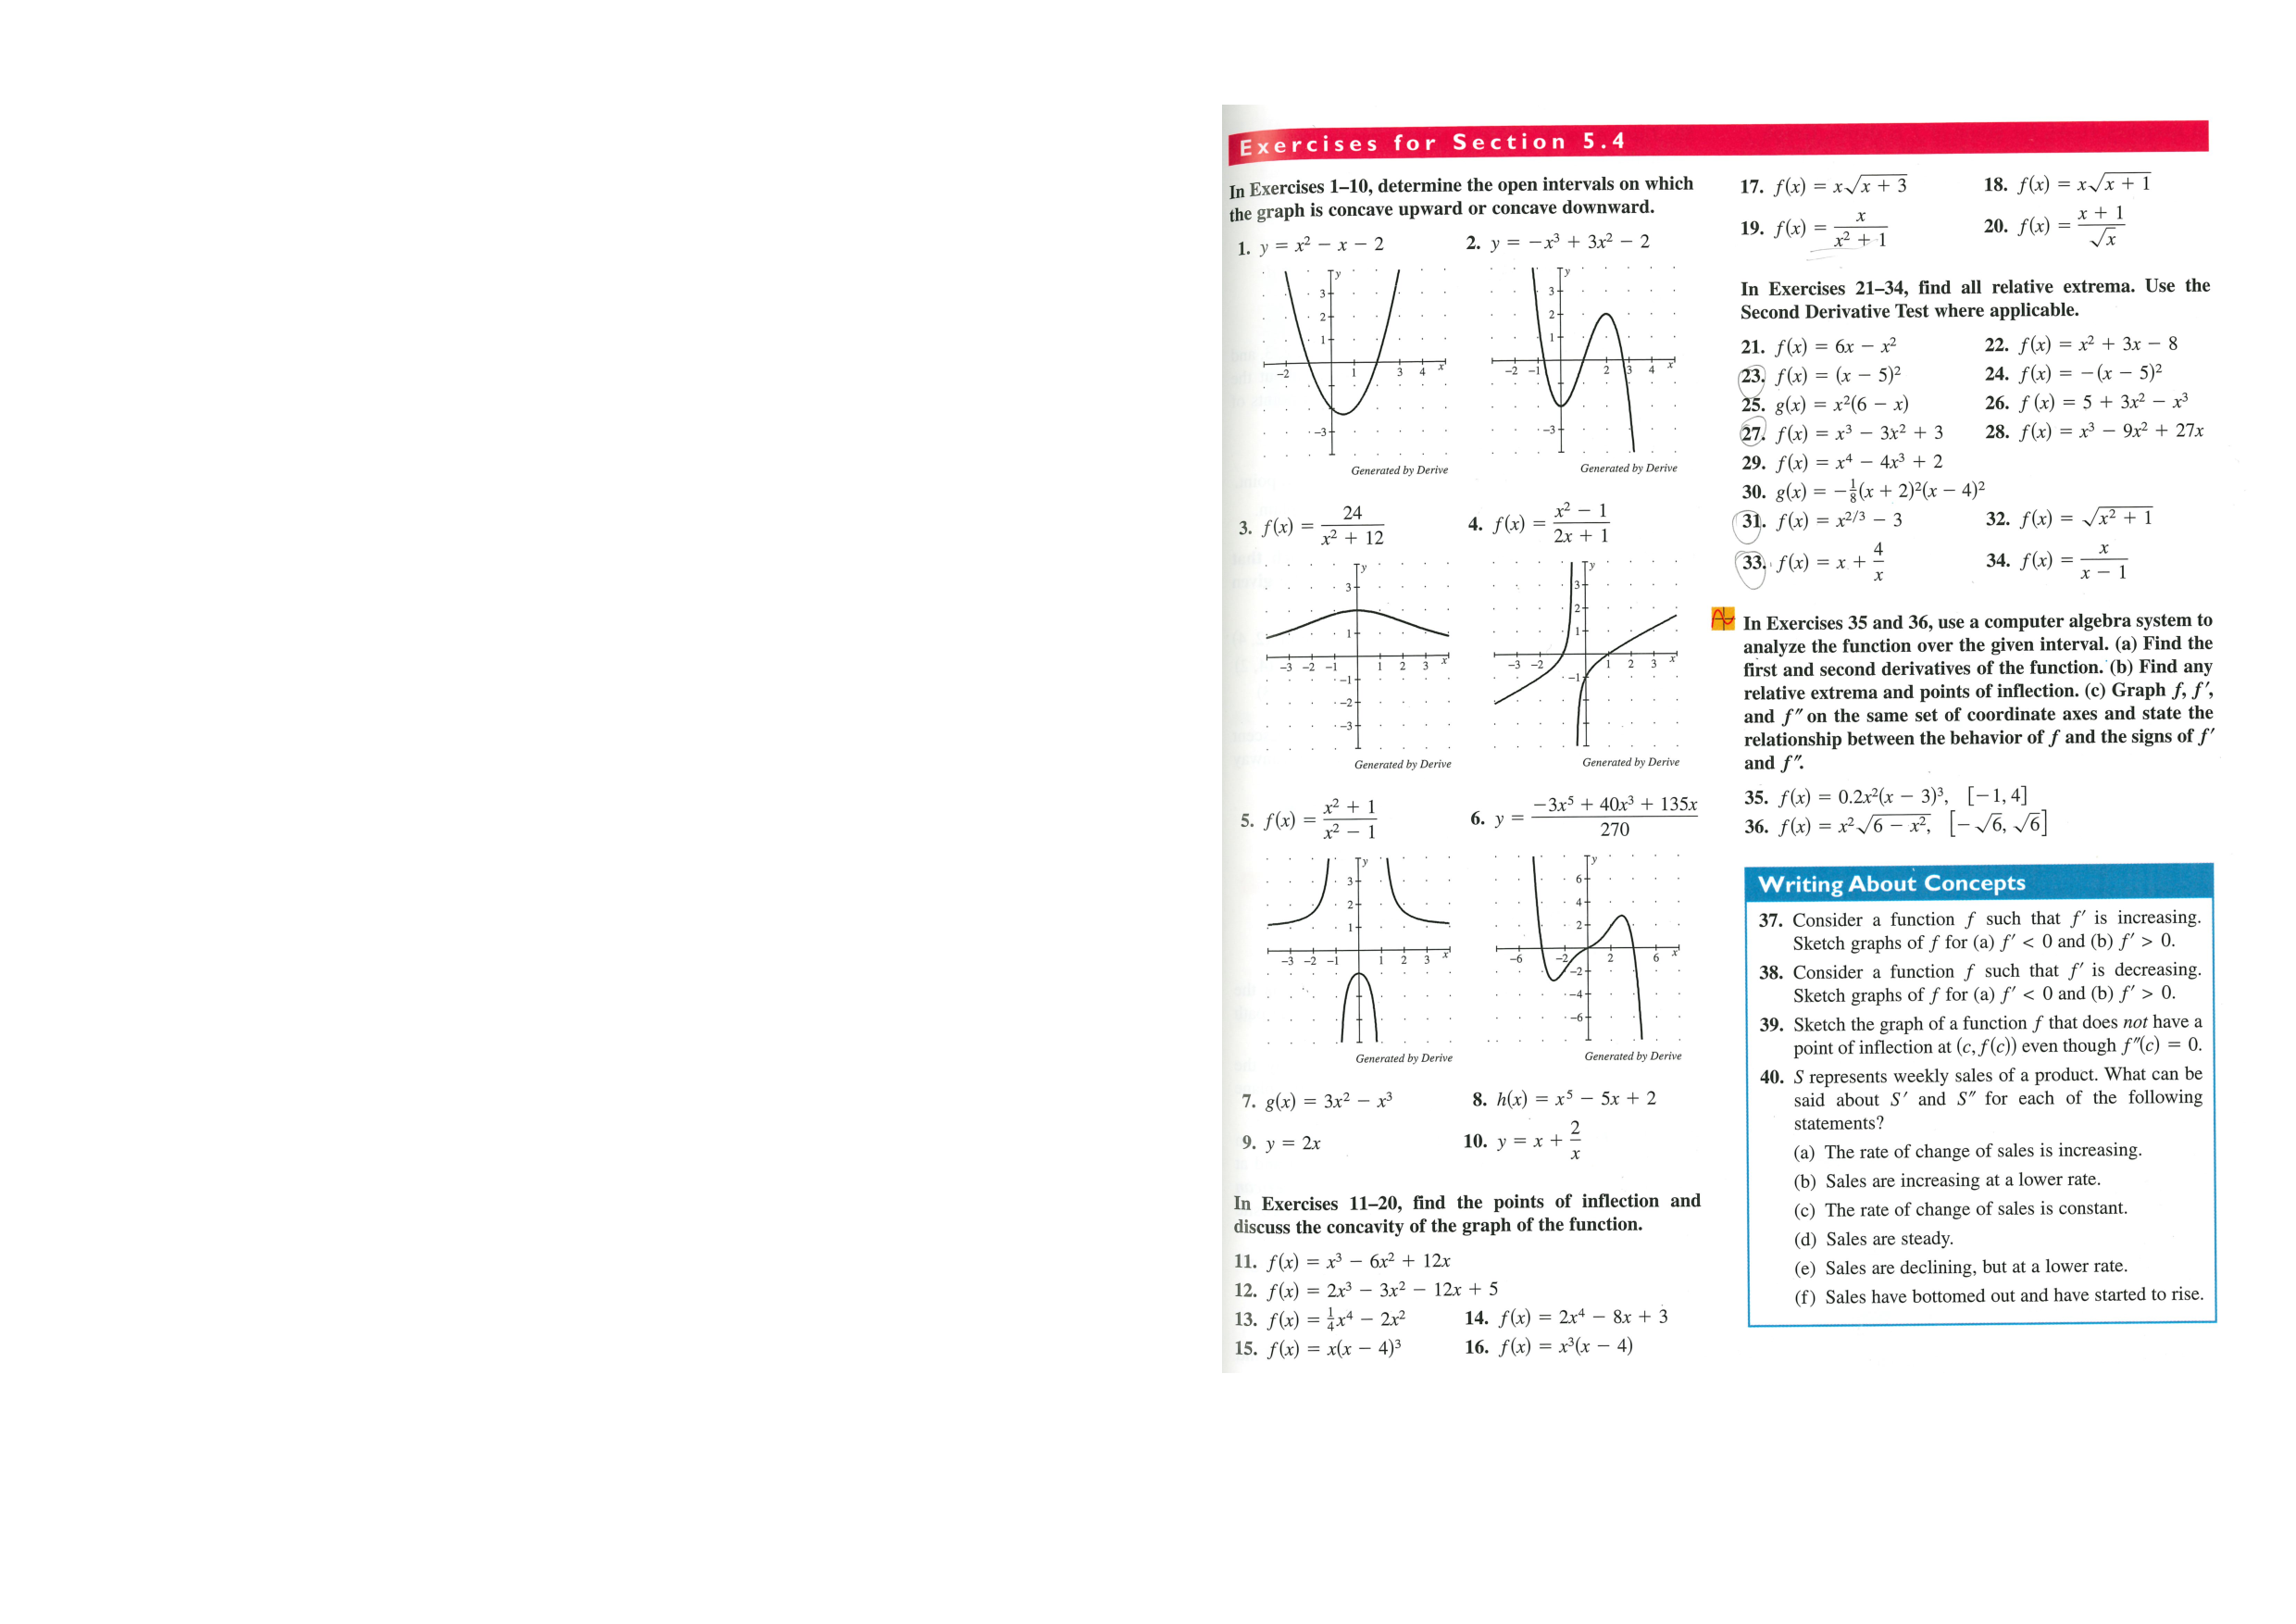
\includegraphics[width=\paperwidth]{\chapdir/0603xA.pdf}}
\newpage
\noindent\makebox[\textwidth]{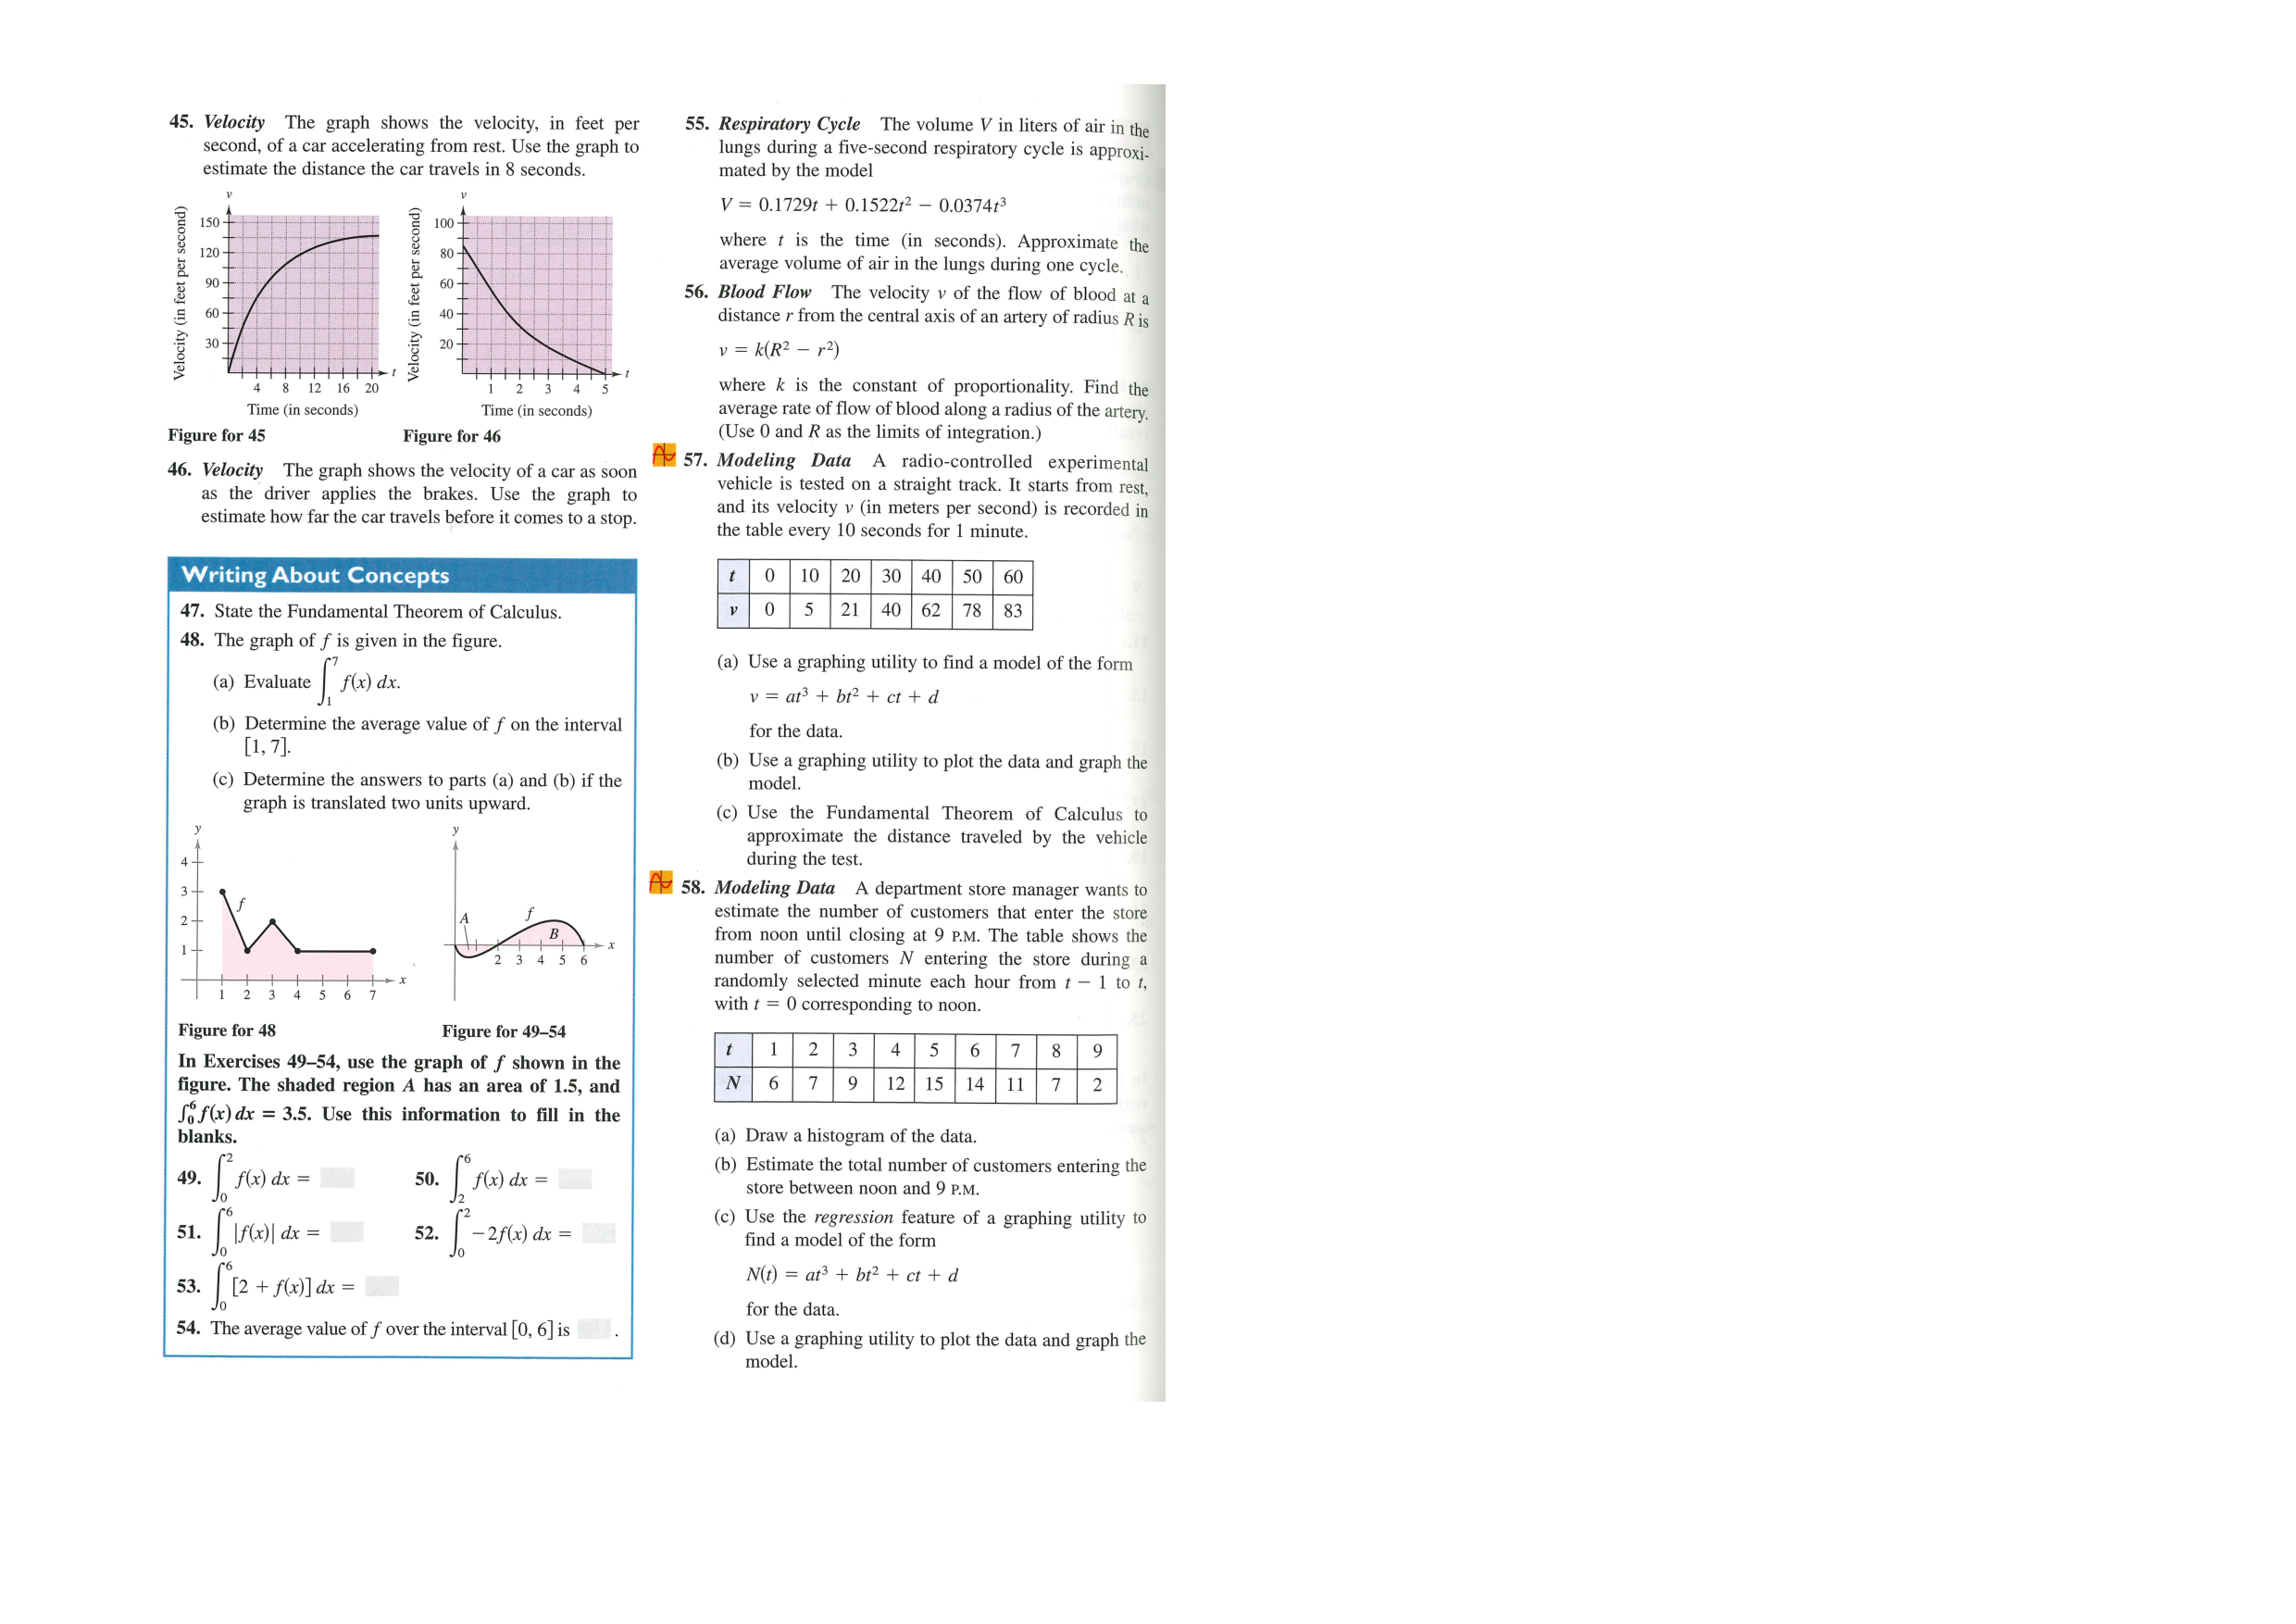
\includegraphics[width=\paperwidth]{\chapdir/0603xB.pdf}}
\newpage
\noindent\makebox[\textwidth]{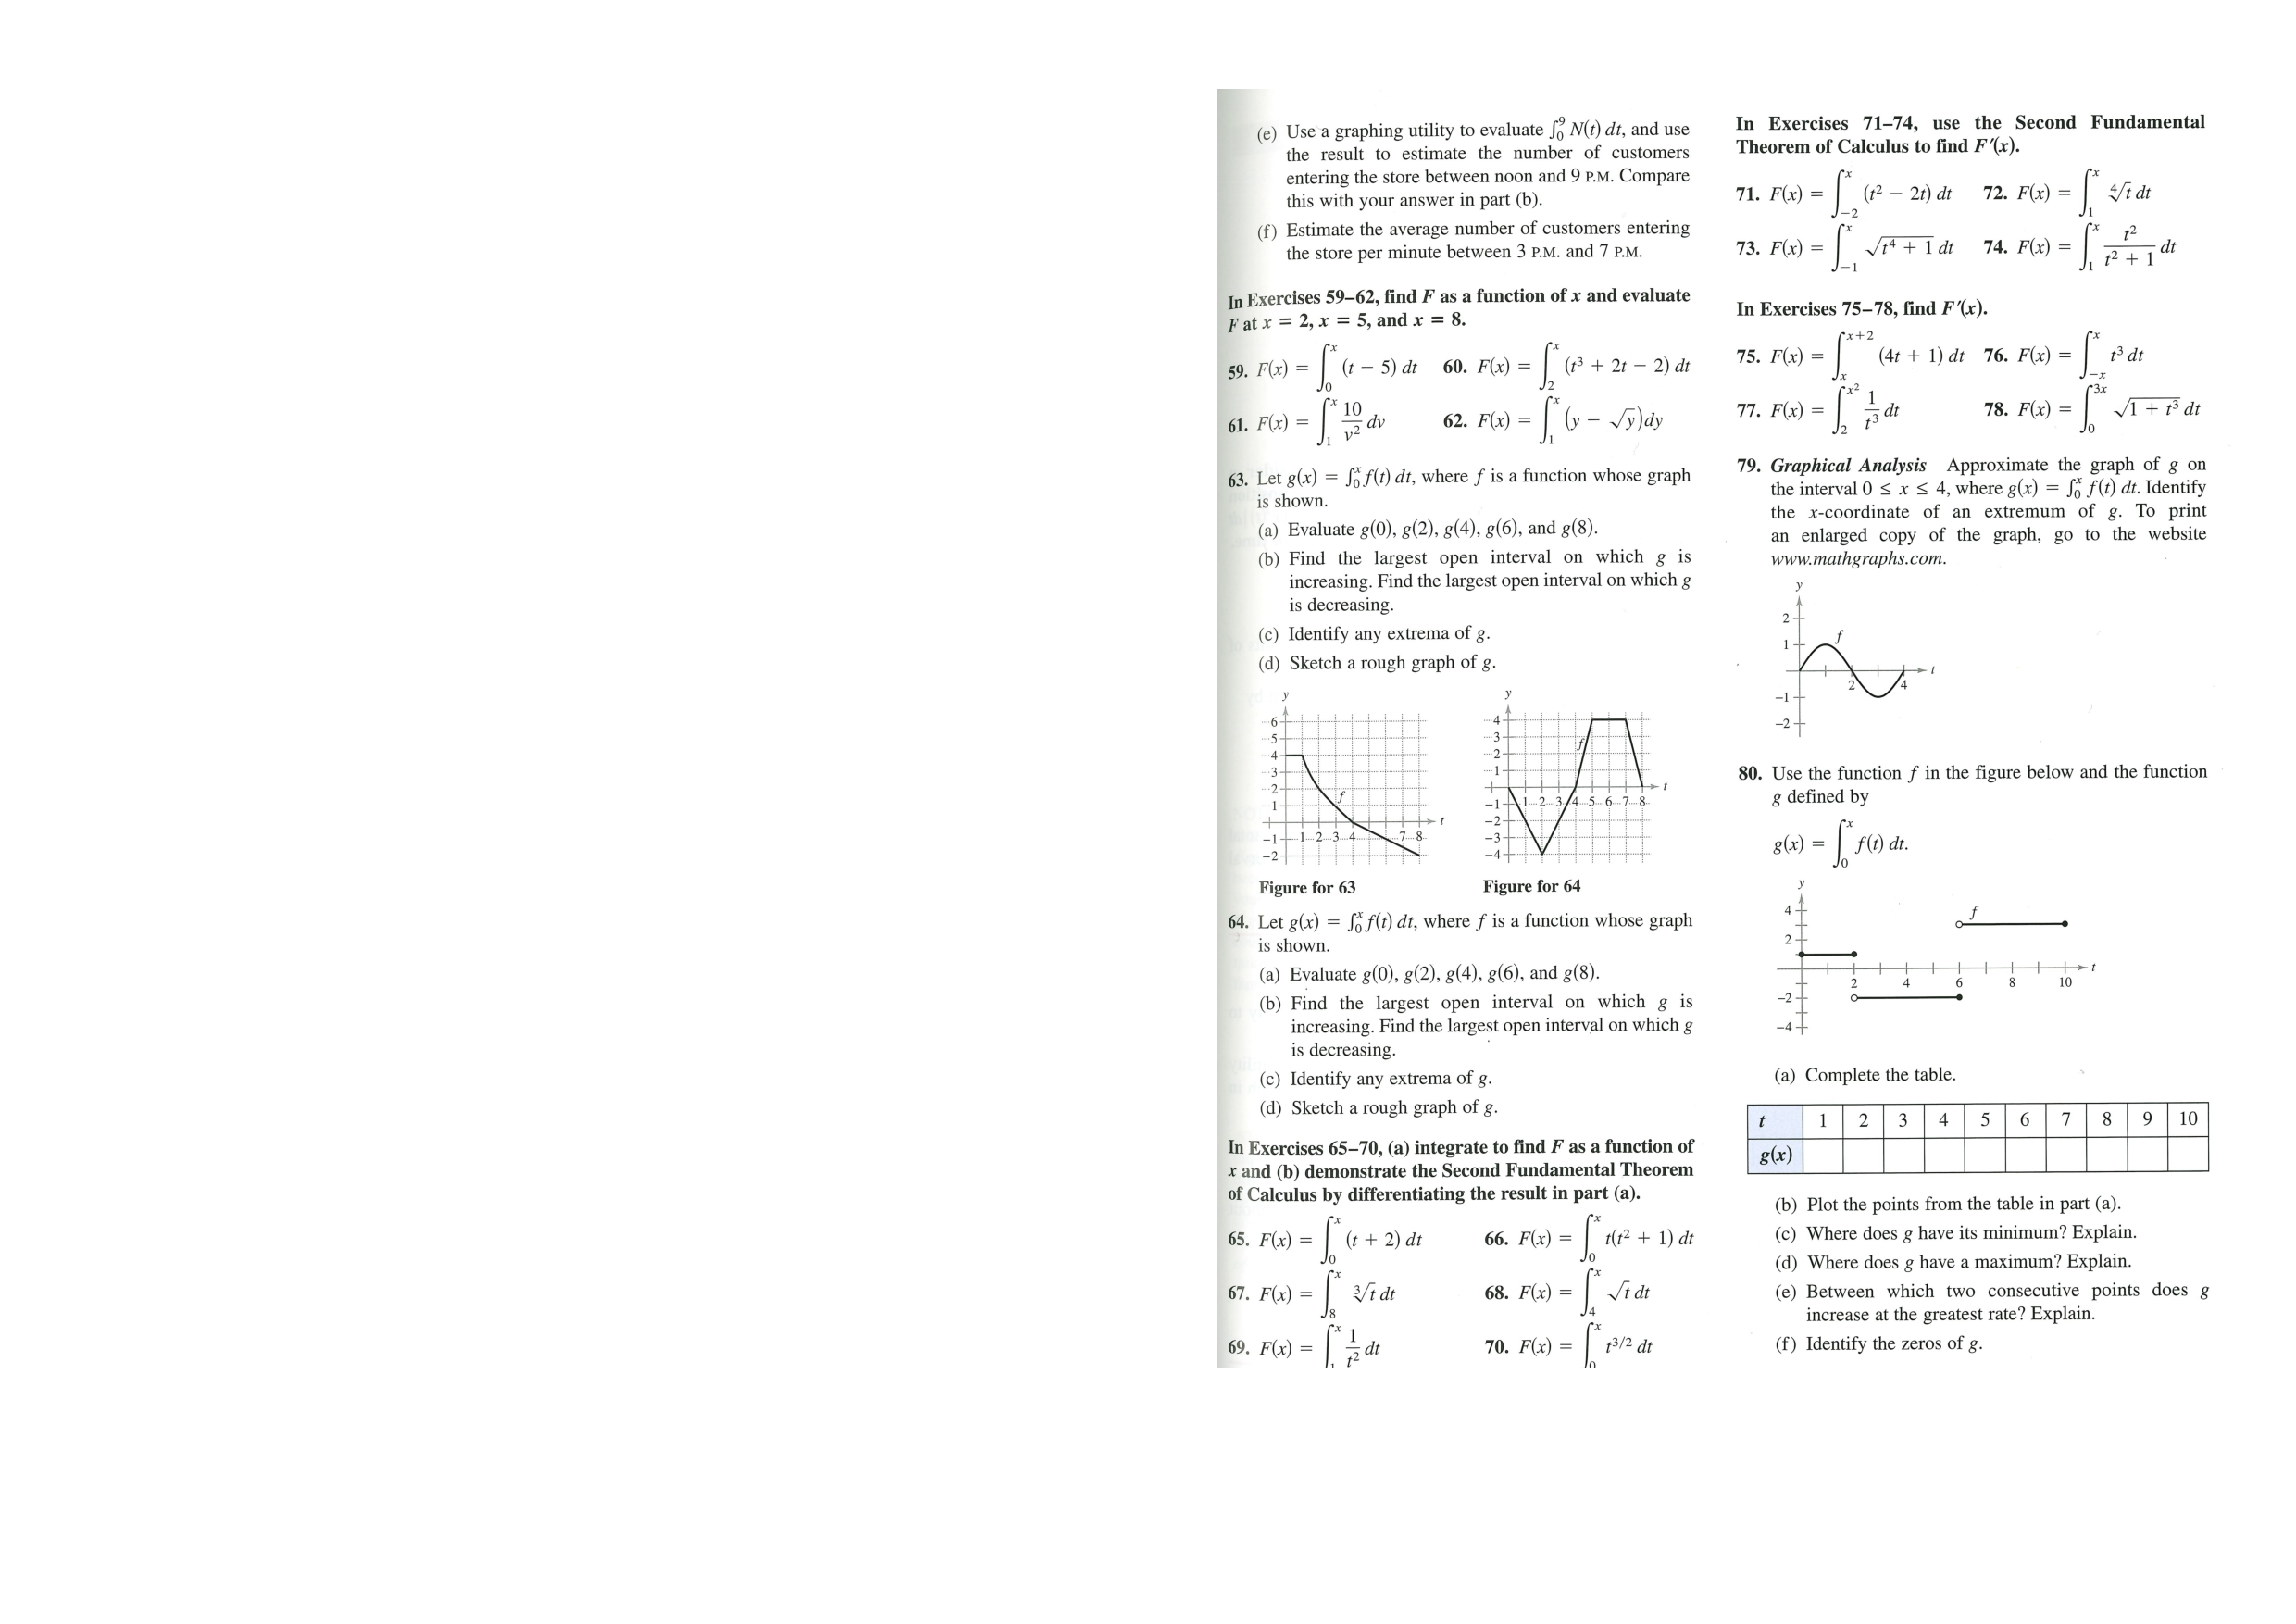
\includegraphics[width=\paperwidth]{\chapdir/0603xC.pdf}}



%									6 - 4
%\newpage
\invisiblesection{Rational Functions}
\subsection{Problems}
\noindent\makebox[\textwidth]{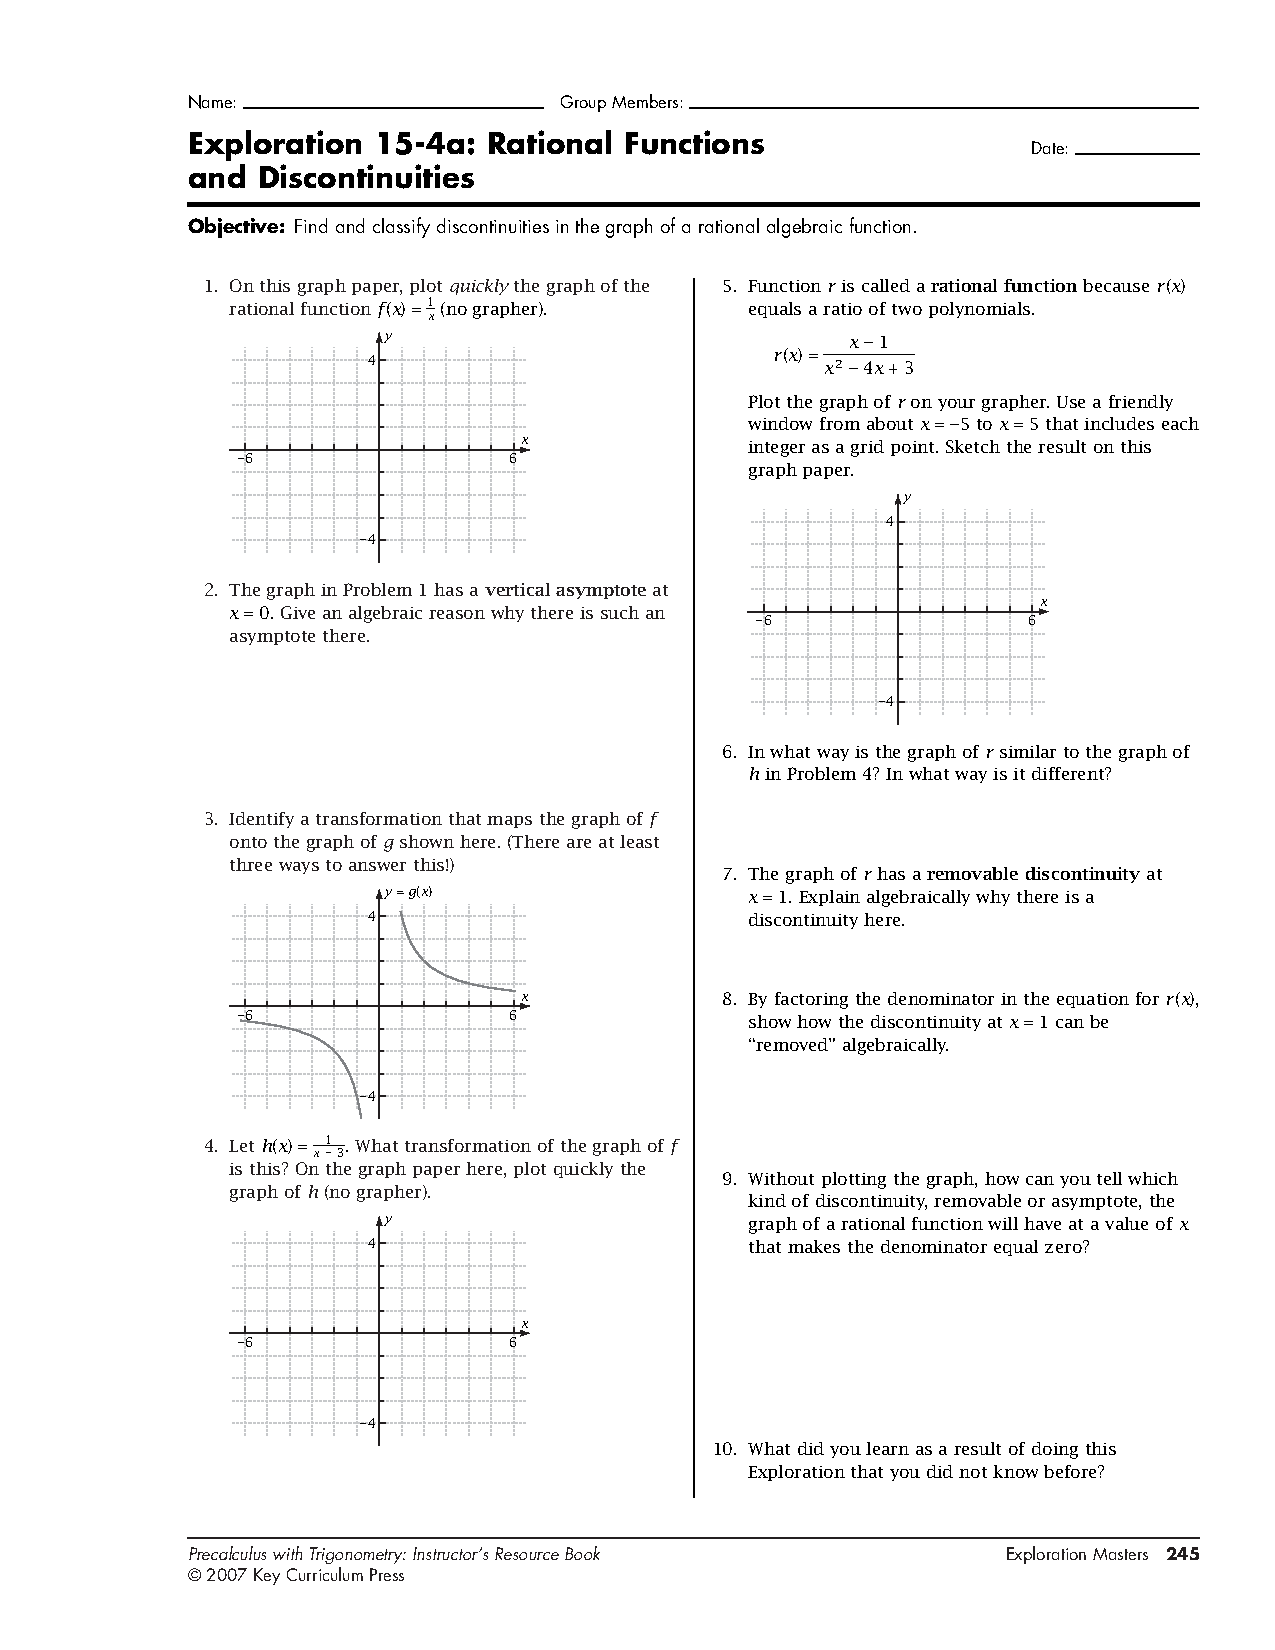
\includegraphics[width=\paperwidth]{\chapdir/0604p.pdf}}
%!TEX root =  ../main.tex

\subsection{Zeros}

\objective{Graph, read, and produce rational functions}


A rational function is one defined by $\frac{f(x)}{g(x)}$ where $f(x)$ and $g(x)$ are both
polynomials.  Rational functions exhibit some common behaviors with polynomials, 
such as $x$-intercepts and one $y$-intercept.  But they also tend to have vertical and
horizontal asymptotes.  The most basic rational function --- $\frac{1}{x}$ --- is, in fact,
a hyperbola, with two branches.  But rational functions can have many more than two
branches, or even just have one.


There are three things one could consider with regard to 0 and a given rational function.
First, the entire quotient could be 0, which would make $x$-intercepts.  Fortunately,
a quotient is only equation to zero when the numerator is equal to zero, meaning
we only need to find when top equation's zeros to find the whole equation's.

When the denominator is equal to zero, much more bizarre behavior emerges.  A vertical
asymptote will occur, though it is not immediately clear if the left and right limits will be
to opposite infinities, or to the same one.  Factoring will make it clear: if the term
has an even multiplicity, the asymptote will be followed to the same infinity.  Otherwise,
one sided-limit will be $\infty$ and the other $-\infty$.

Lastly, we should consider what happens when we make the argument 0.  A $y$-intercept
is always a coordinate with the appearance $(0,y_0)$, so plugging in 0 is an efficient way
to find it.

Each of these three techniques for various ``zero's'', assumes that it is not occurring when
function is in an indeterminate form.  Holes and asymptotes can prevent intercepts from 
actually occurring, and obfuscate one another

\subsection{Horizontal Asymptotes}
If a rational function looks like a fraction, a ratio, a quotient, that's because it is!  Just as
a polynomial looks more and more like an integer power function the further out one zooms,
so too a rational function will look more like the results if one simply divides the numerator
by the denominator.

Consider the function $r(x) = \dfrac{2x^2-4x-6}{x^2+x-2}$.  In the big picture, 
it is a simple division problem.  Ultimately, we want to know $lim_{x\rightarrow\infty} 
r(x)$:

\polylongdiv{2x^2-4x-6}{x^2+x-2}

and so the question becomes equivalent to 

$$
\lim_{x\rightarrow\infty} 2-\frac{6x+2}{x^2+x-2}
$$

which is two.

We might have spared ourselves the work of polynomial long division by contrasting the degree
of the numerator and denominator beforehand.  Which has greater degree?
\begin{itemize}
\item[denominator] the long term behavior can be modeled by a horizontal asymptote at $y=0$
\item[neither] the long tern behavior will still be a horizontal asymptote at $y=\frac{a}{b}$, where $a$ and $b$ are the leading terms of the numerator and denominator respectively
\item[numerator] polynomial division cannot be avoided, and the long-run behavior trends towards an asymptote at $y=$ the quotient, ignoring the remainder
\end{itemize}

\subsection{Signs}
Rational functions are among the hardest for graphers to correctly display.  
Even large computers can display misleading results if the window is not correctly 
pre-programmed.  If it is necessary to map out the sign of the function beforehand,
a tabular approach can be very helpful.  We will combine a number line and a table
into a new kind of grid, using the following function as an example:

$$Y_1=\frac{x+1}{(10x-1)^2}$$

\begin{figure}[h]
\begin{centering}
\begin{tikzpicture}

\matrix (m) [matrix of math nodes, 
             column sep=0cm, row sep=0pt,
     nodes={text width=15mm, align=center, 
            text height=3ex, text depth=1.5ex}]
{
(x+1)       &   -   &   +   &   +   \\
(10x-1)^2    &   +   &   +   &   +   \\
\textbf{Q}        &   \textbf{-}  &  \textbf{+}    &  \textbf{+}    \\
};
\draw  (m-1-1.north west) -- (m-1-4.north east);
\draw (m-2-1.north west) -- (m-2-4.north east);
\draw (m-3-1.north west) -- (m-3-4.north east);
\draw (m-3-1.south west) -- (m-3-4.south east);

\draw  (m-1-1.north east) -- (m-3-1.south east);
\draw (m-1-2.north east) -- (m-3-2.south east);
\draw (m-1-3.north east) -- (m-3-3.south east);
\draw (m-1-4.north east) -- (m-3-4.south east);

\node[above] at (m-1-2.north east) {$-1$};
\node[above] at (m-1-3.north east) {$0.1$};

\node at (m-1-2.east) {$0$};
\node at (m-2-2.east) {$+$};
\node at (m-3-2.east) {\textbf{0}};

\node at (m-1-3.east) {$+$};
\node at (m-2-3.east) {$0$};
\node at (m-3-3.east) {\textbf{$\infty$}};
\end{tikzpicture}
\caption{A sign table and number-line combination}
\end{centering}
\end{figure}

The table is made by writing the factors of the numerator and denominator down the
left.  The bottom row is the function itself, which is the quotient of the rest.  Across 
the top, you will need a division for each of the zeros of the factors and room
for all the spaces in-between and around.  On the lines, write the zero's if the factor
is zero there, or just the sign.  To complete the bottom, simply remember the
rules of  signs:

\begin{enumerate}
\item a positive multiplied or divided by a positive is a positive
\item a negative multiplied or divided by a negative is a negative
\item a negative multiplied or divided by a negative is positive
\end{enumerate}

The zero's require only a little more thought.  A zero in the numerator
makes the entire quotient zero.  If a zero in the numerator is surrounded by
like signs, then either side of the vertical asymptote will go to that sign infinity.
If the signs disagree, then both infinities will be approached, each from the
side matching their sign.

\begin{figure}
\begin{centering}
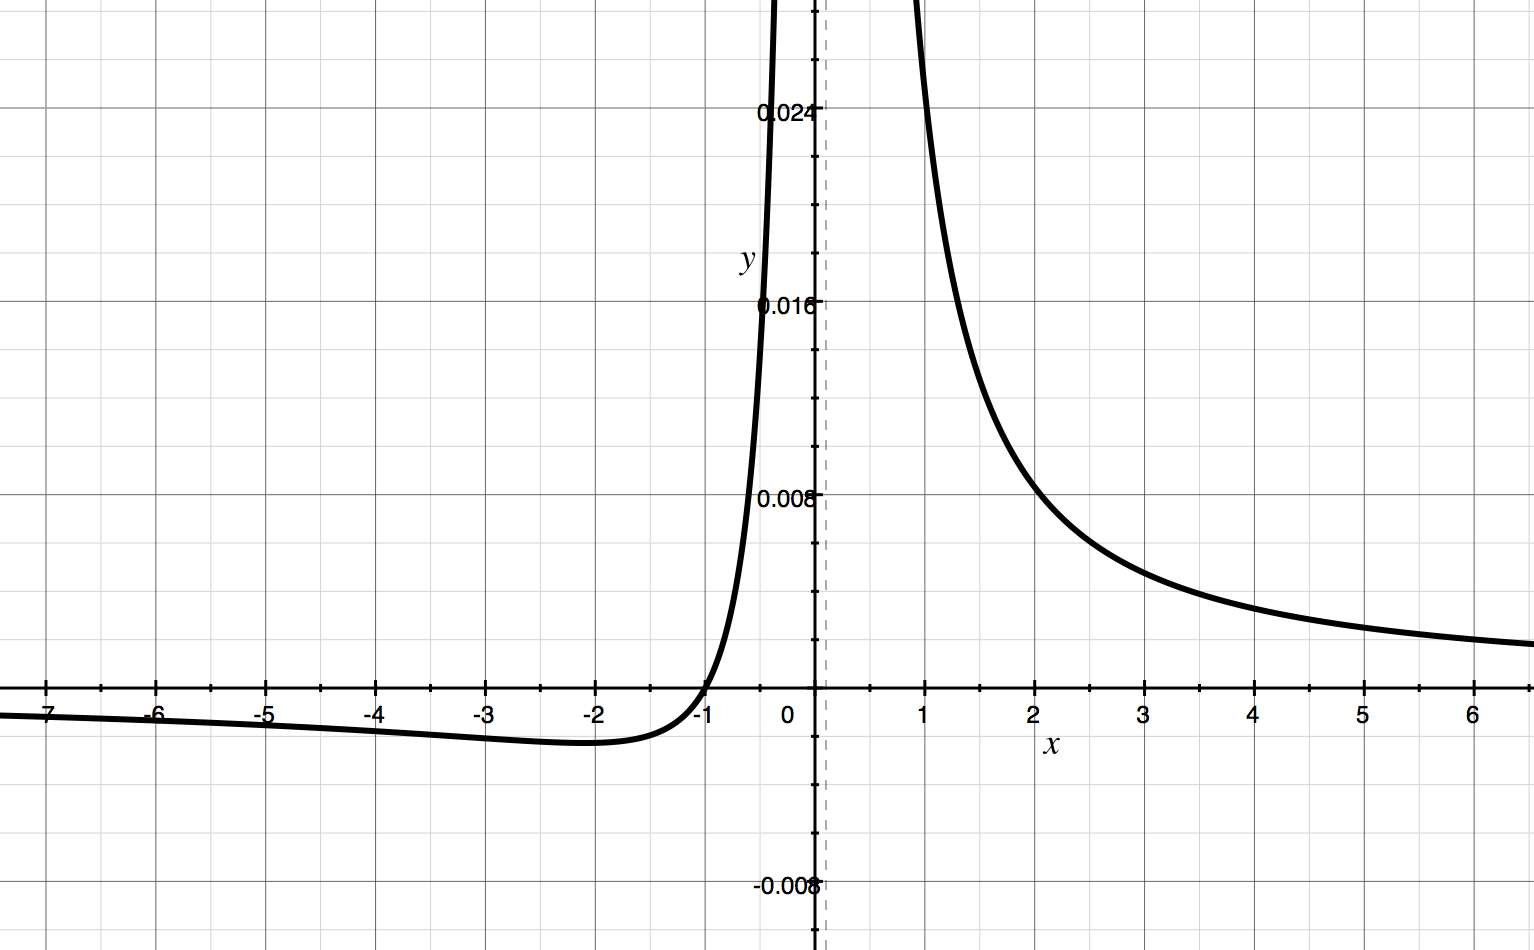
\includegraphics[scale=0.3]{\chapdir/pics/verticalasymptote}
\caption{An appropriately zoomed in graph of $\frac{x+1}{(10x-1)^2}$}
\end{centering}
\end{figure}

With this much more appropriate window, we can see that there is a local minimum,
perhaps in the vicinity of $x=-2$.  If it indeed occurs at a rational number, there is no
reason to find the derivative by hand with the TI-8* will do it for us!

\index{TI-8*!graph derivatives}
Set $Y_2$ to be \texttt{nDeriv(Y$_1$(X),X,X)} or $\left.\frac{d}{dx}(Y_1(X))\right|_{X=X}$, 
depending upon your model of TI-8*.  (nDerive is choice 8 under 
\Touche[style=function,principal=math].)  It seems have a
zero near 2.  The function is clearly concave and derivative is increasing, so it should be
a local minimum.  Using ZERO (under 
\Touche[style=function,principal=trace,fontsize=7pt,position=0.9]
), we find it to be exactly -2.1.  Plugging
back into the original equation, we get $\frac{-1.1}{484}$, which $\triangleright$FRAC
converts to $-\frac{1}{440}$.

\newpage
\subsection{Exercises}
\noindent\makebox[\textwidth]{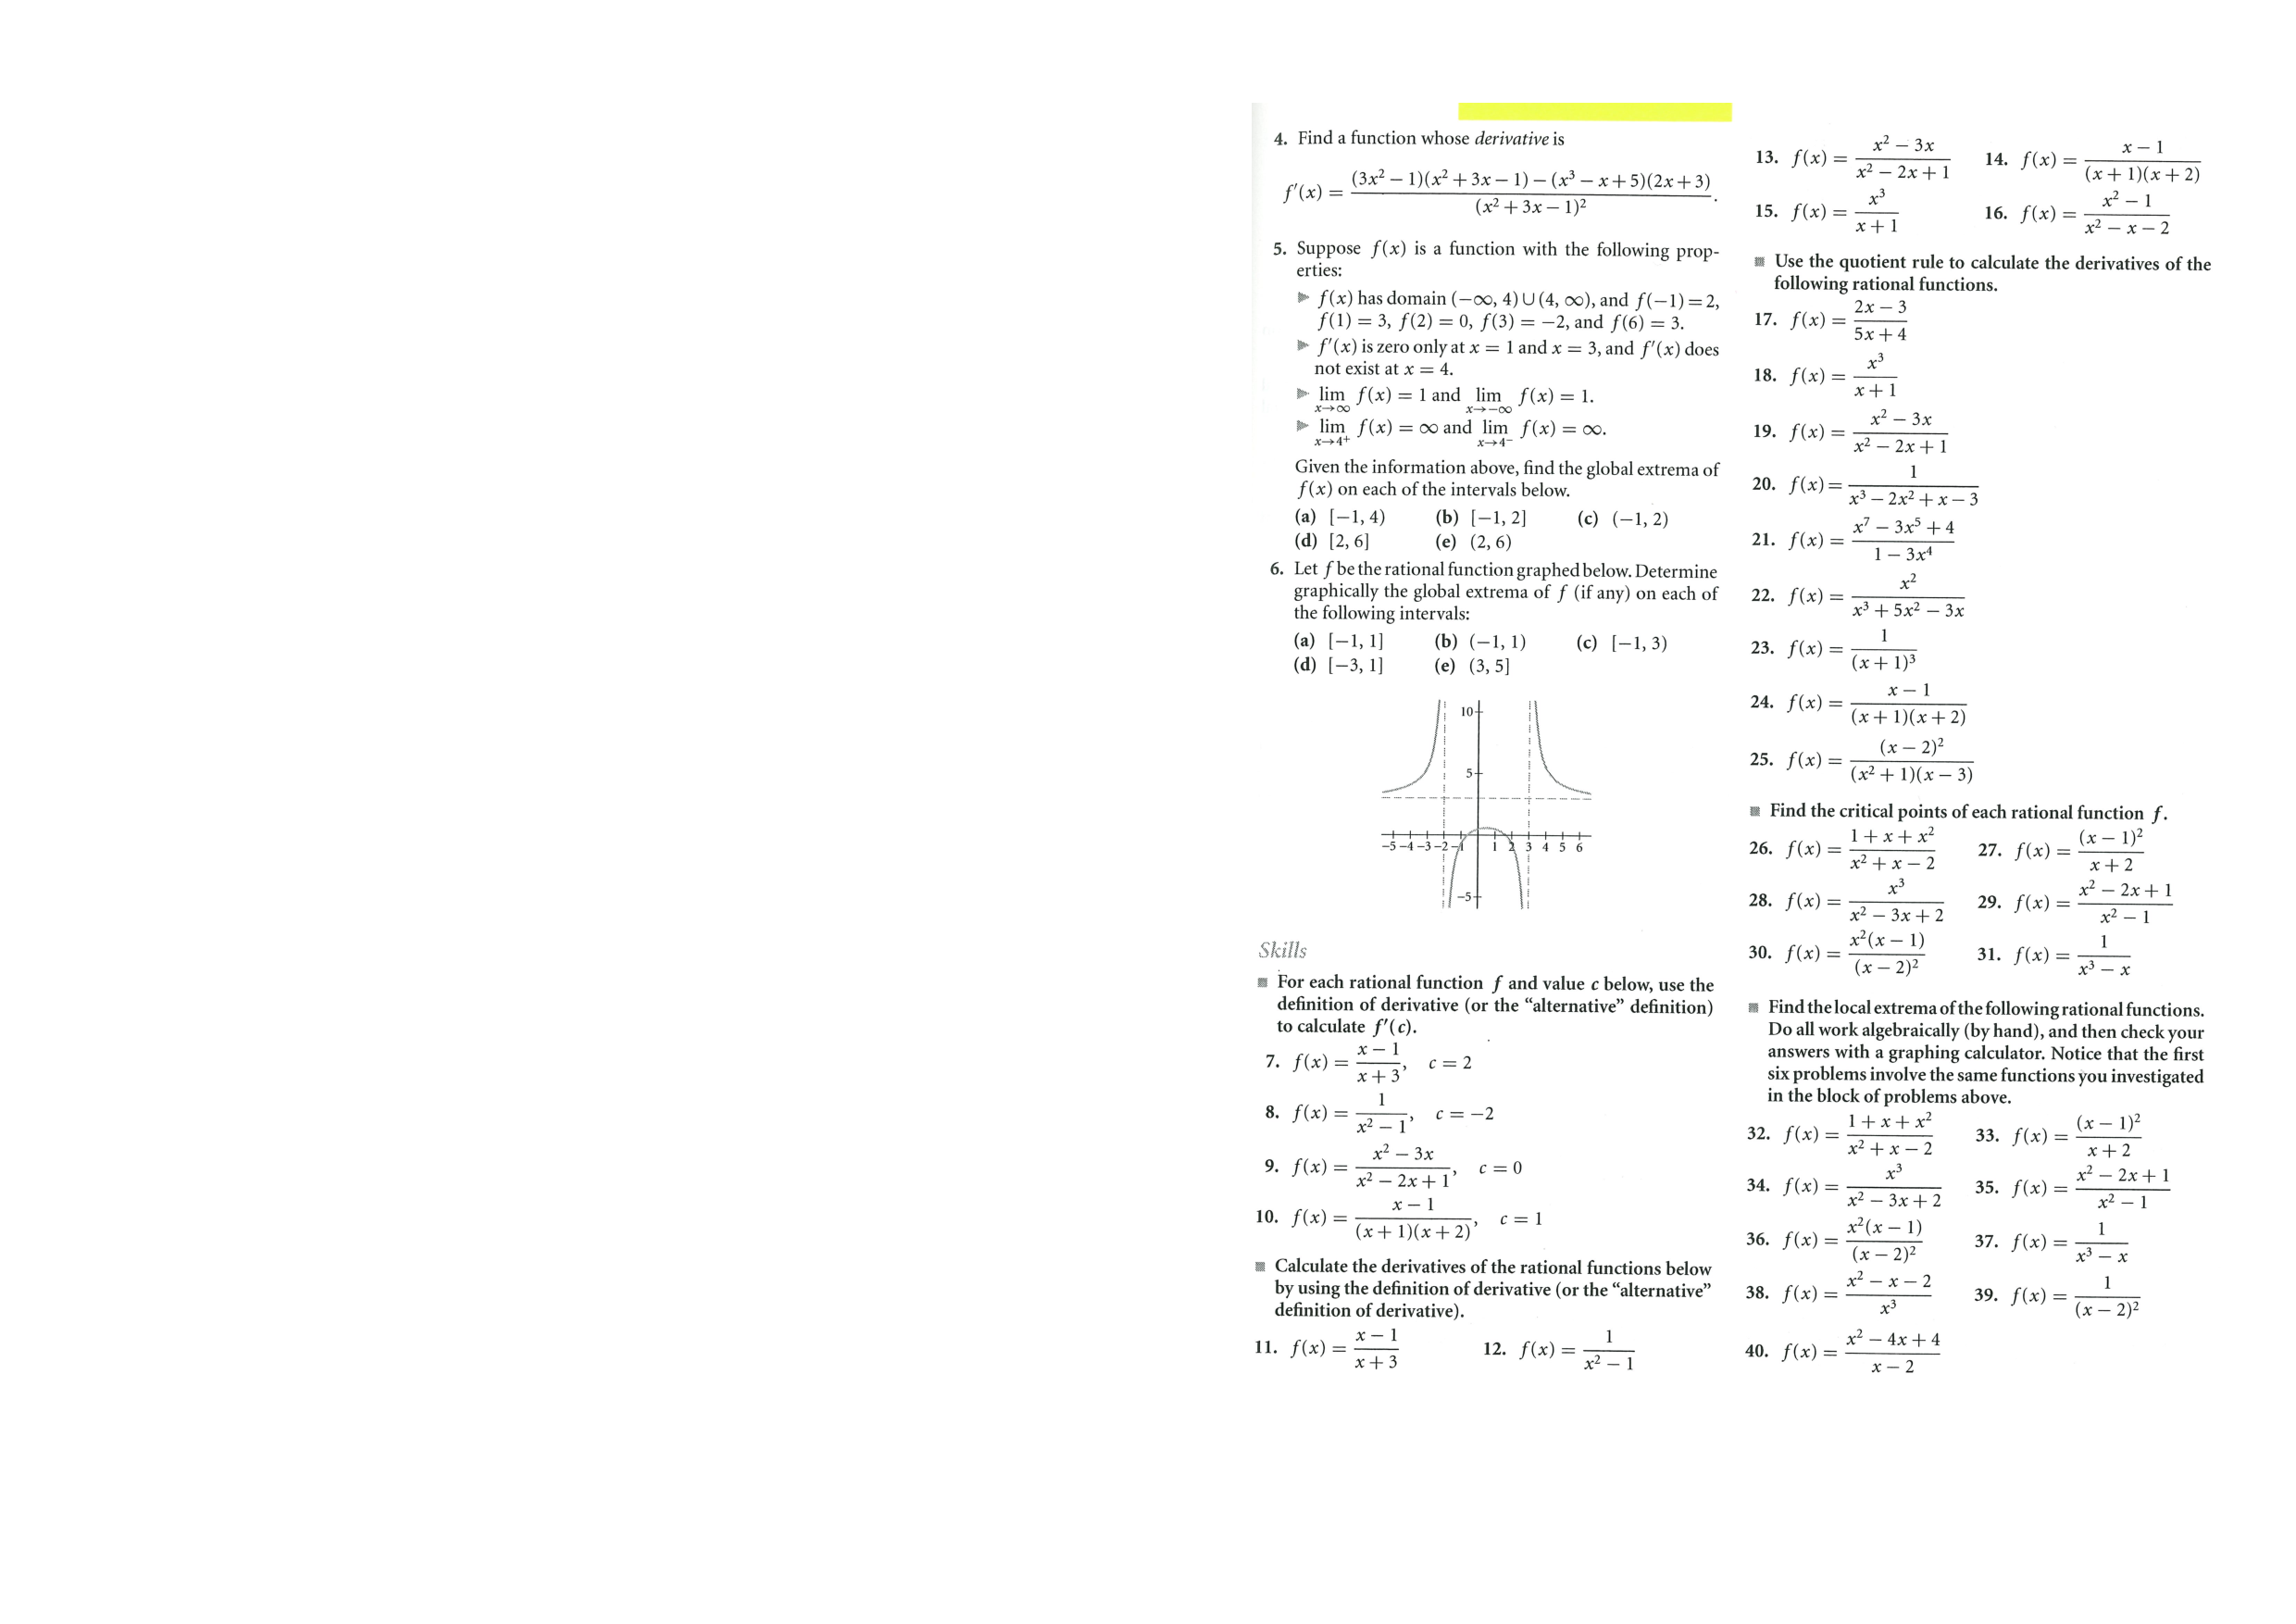
\includegraphics[width=\paperwidth]{\chapdir/0604xA.pdf}}
\newpage
\noindent\makebox[\textwidth]{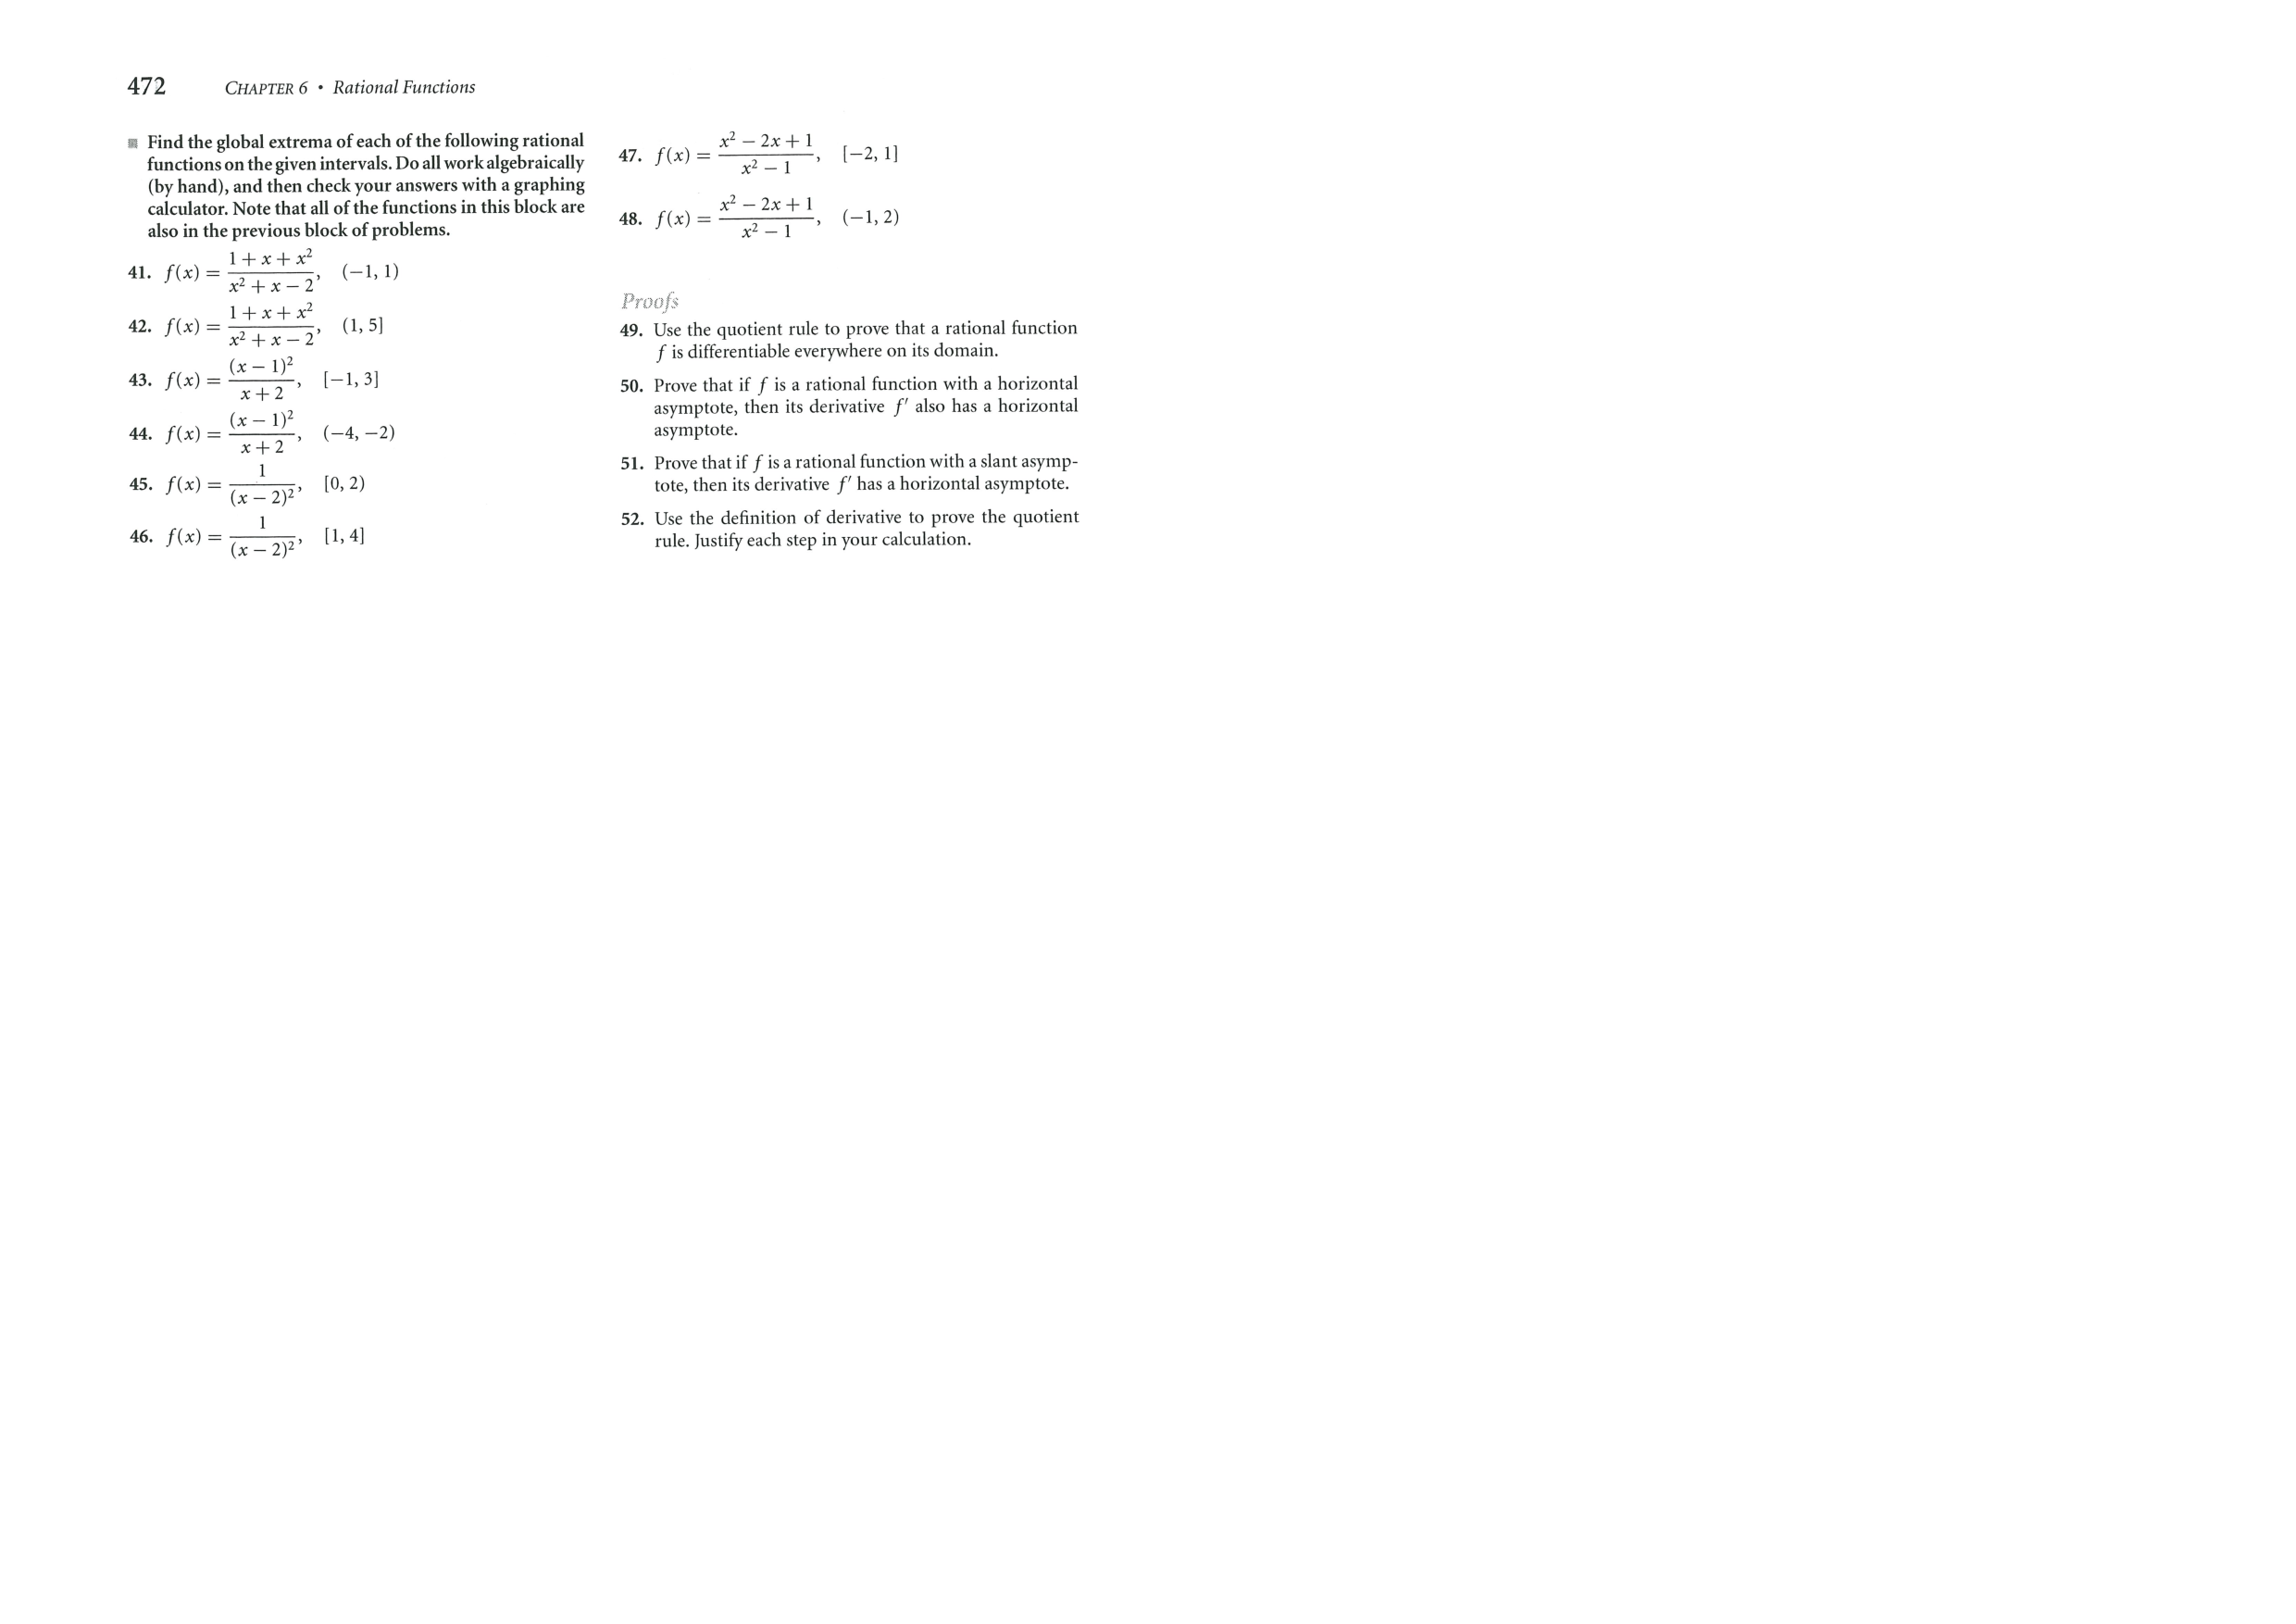
\includegraphics[width=\paperwidth]{\chapdir/0604xB.pdf}}
\newpage
\noindent\makebox[\textwidth]{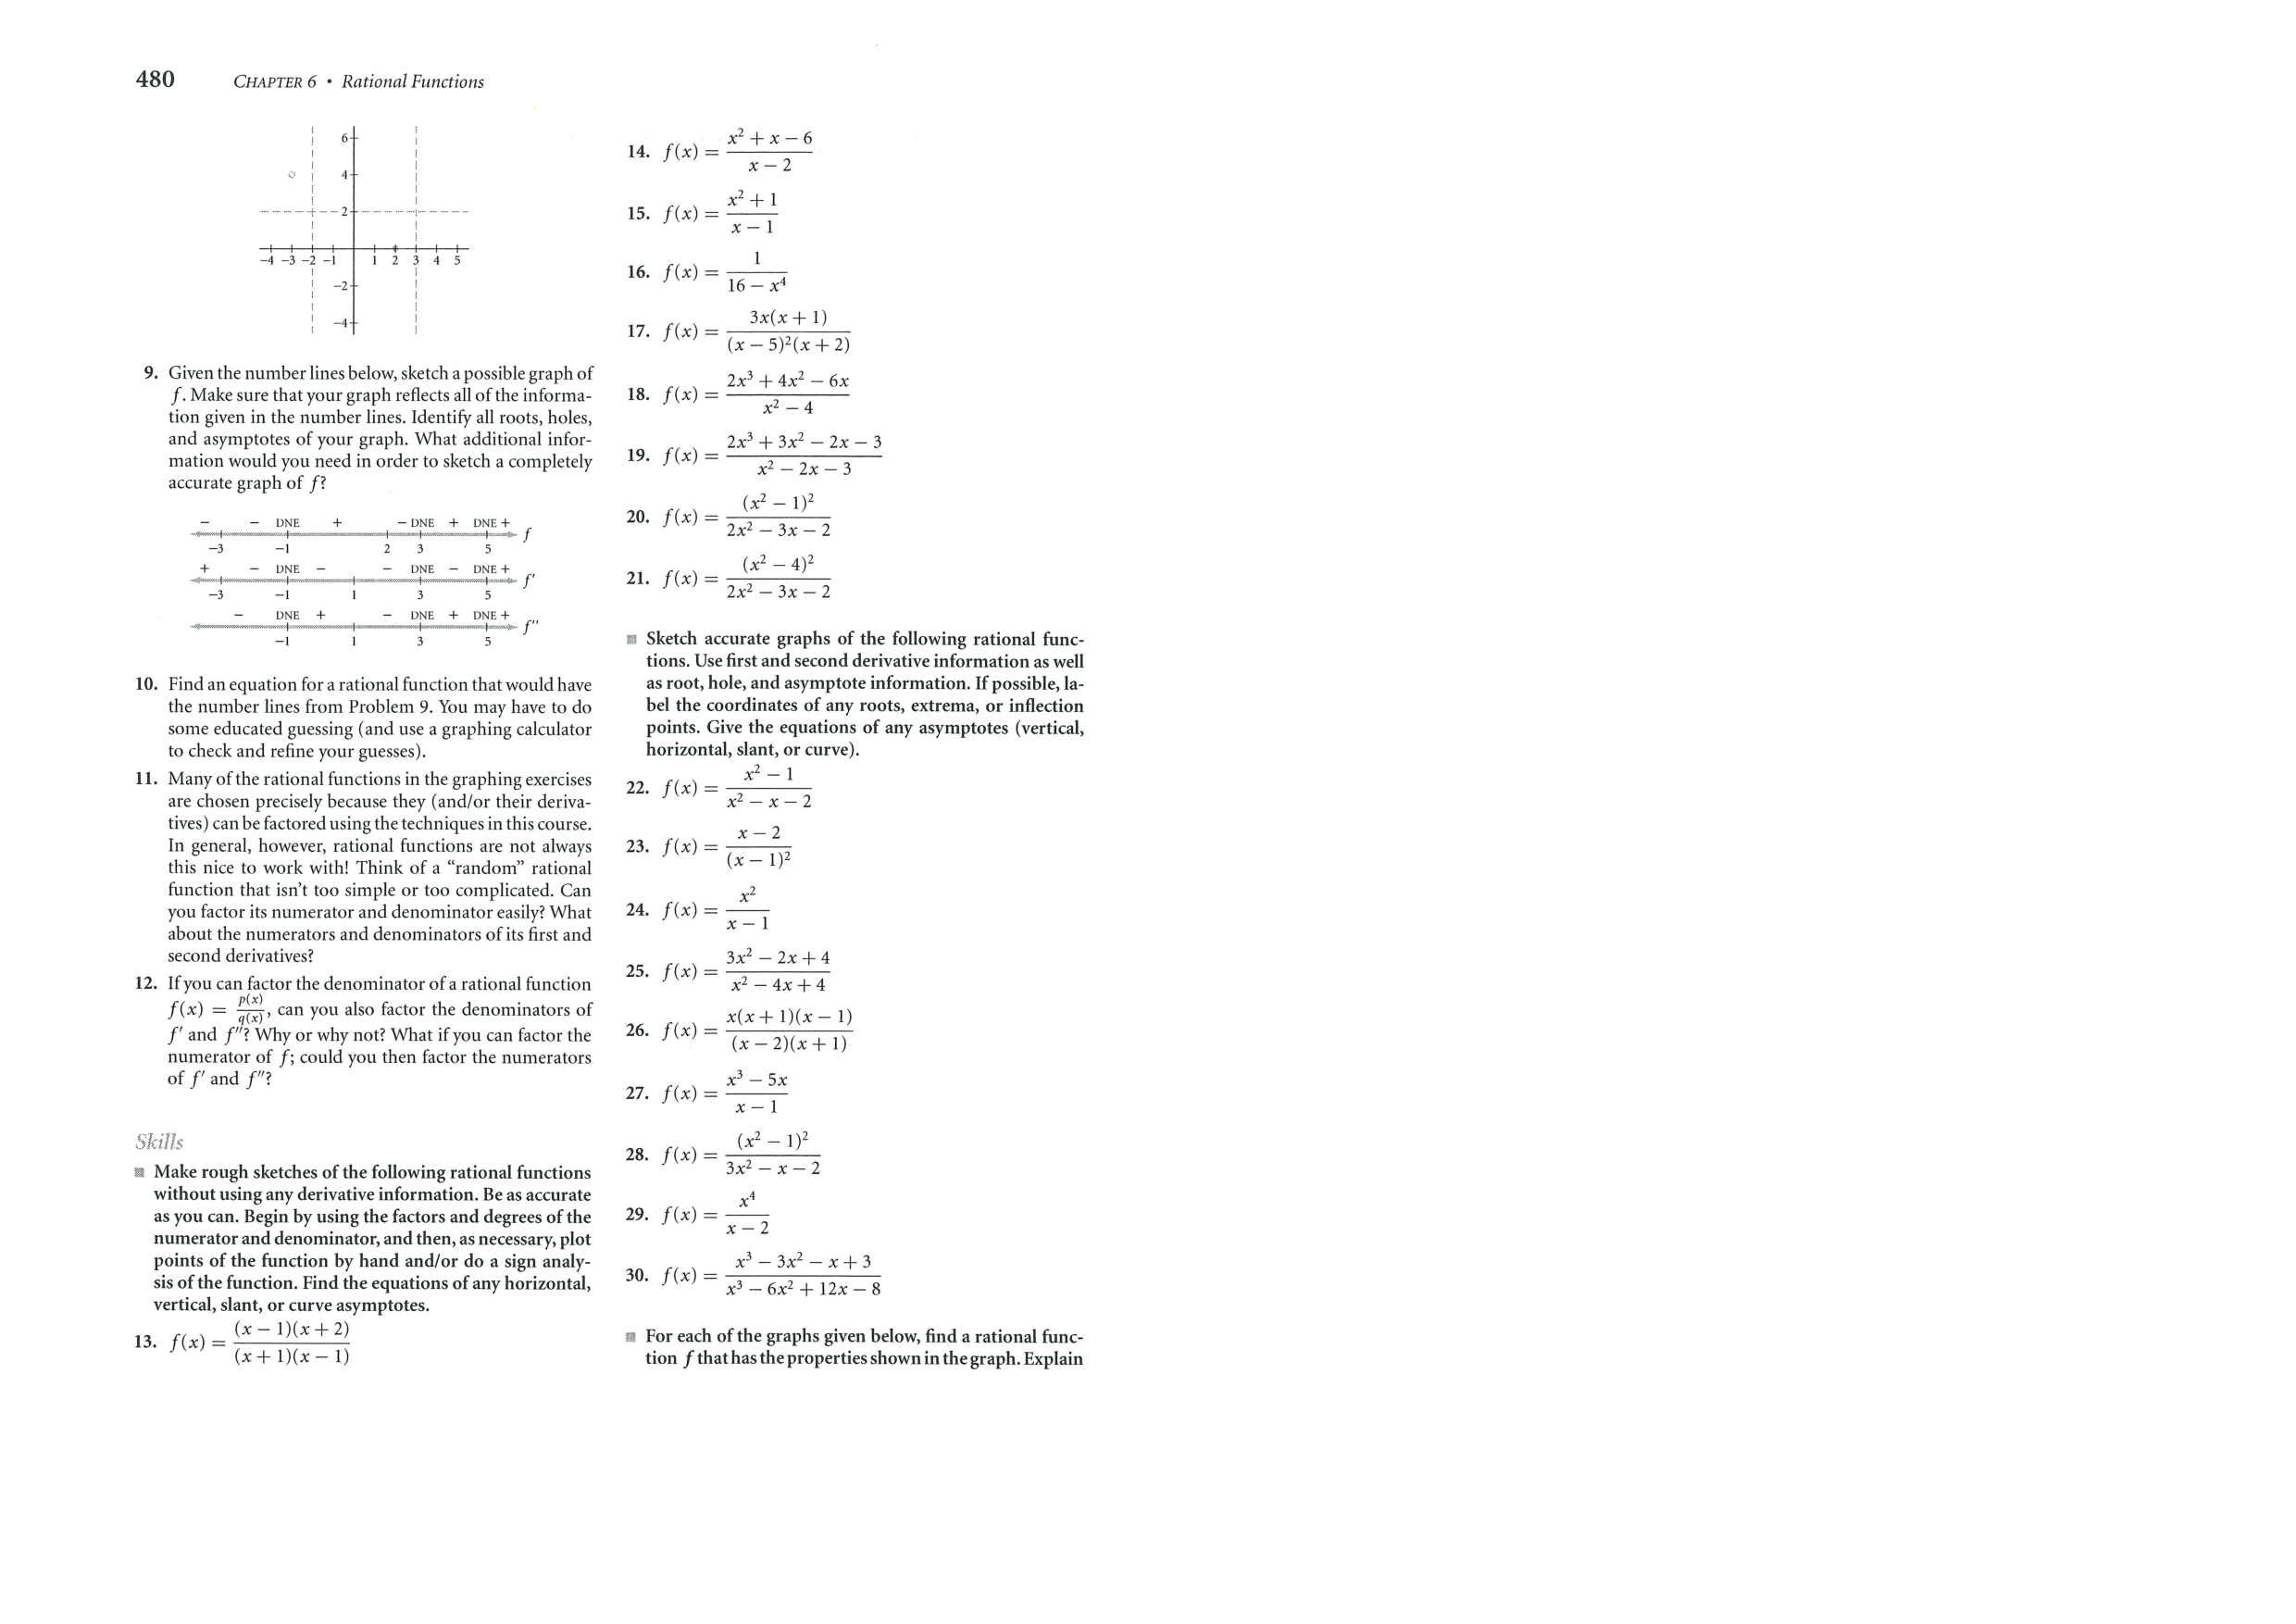
\includegraphics[width=\paperwidth]{\chapdir/0604xC.pdf}}
\newpage
\noindent\makebox[\textwidth]{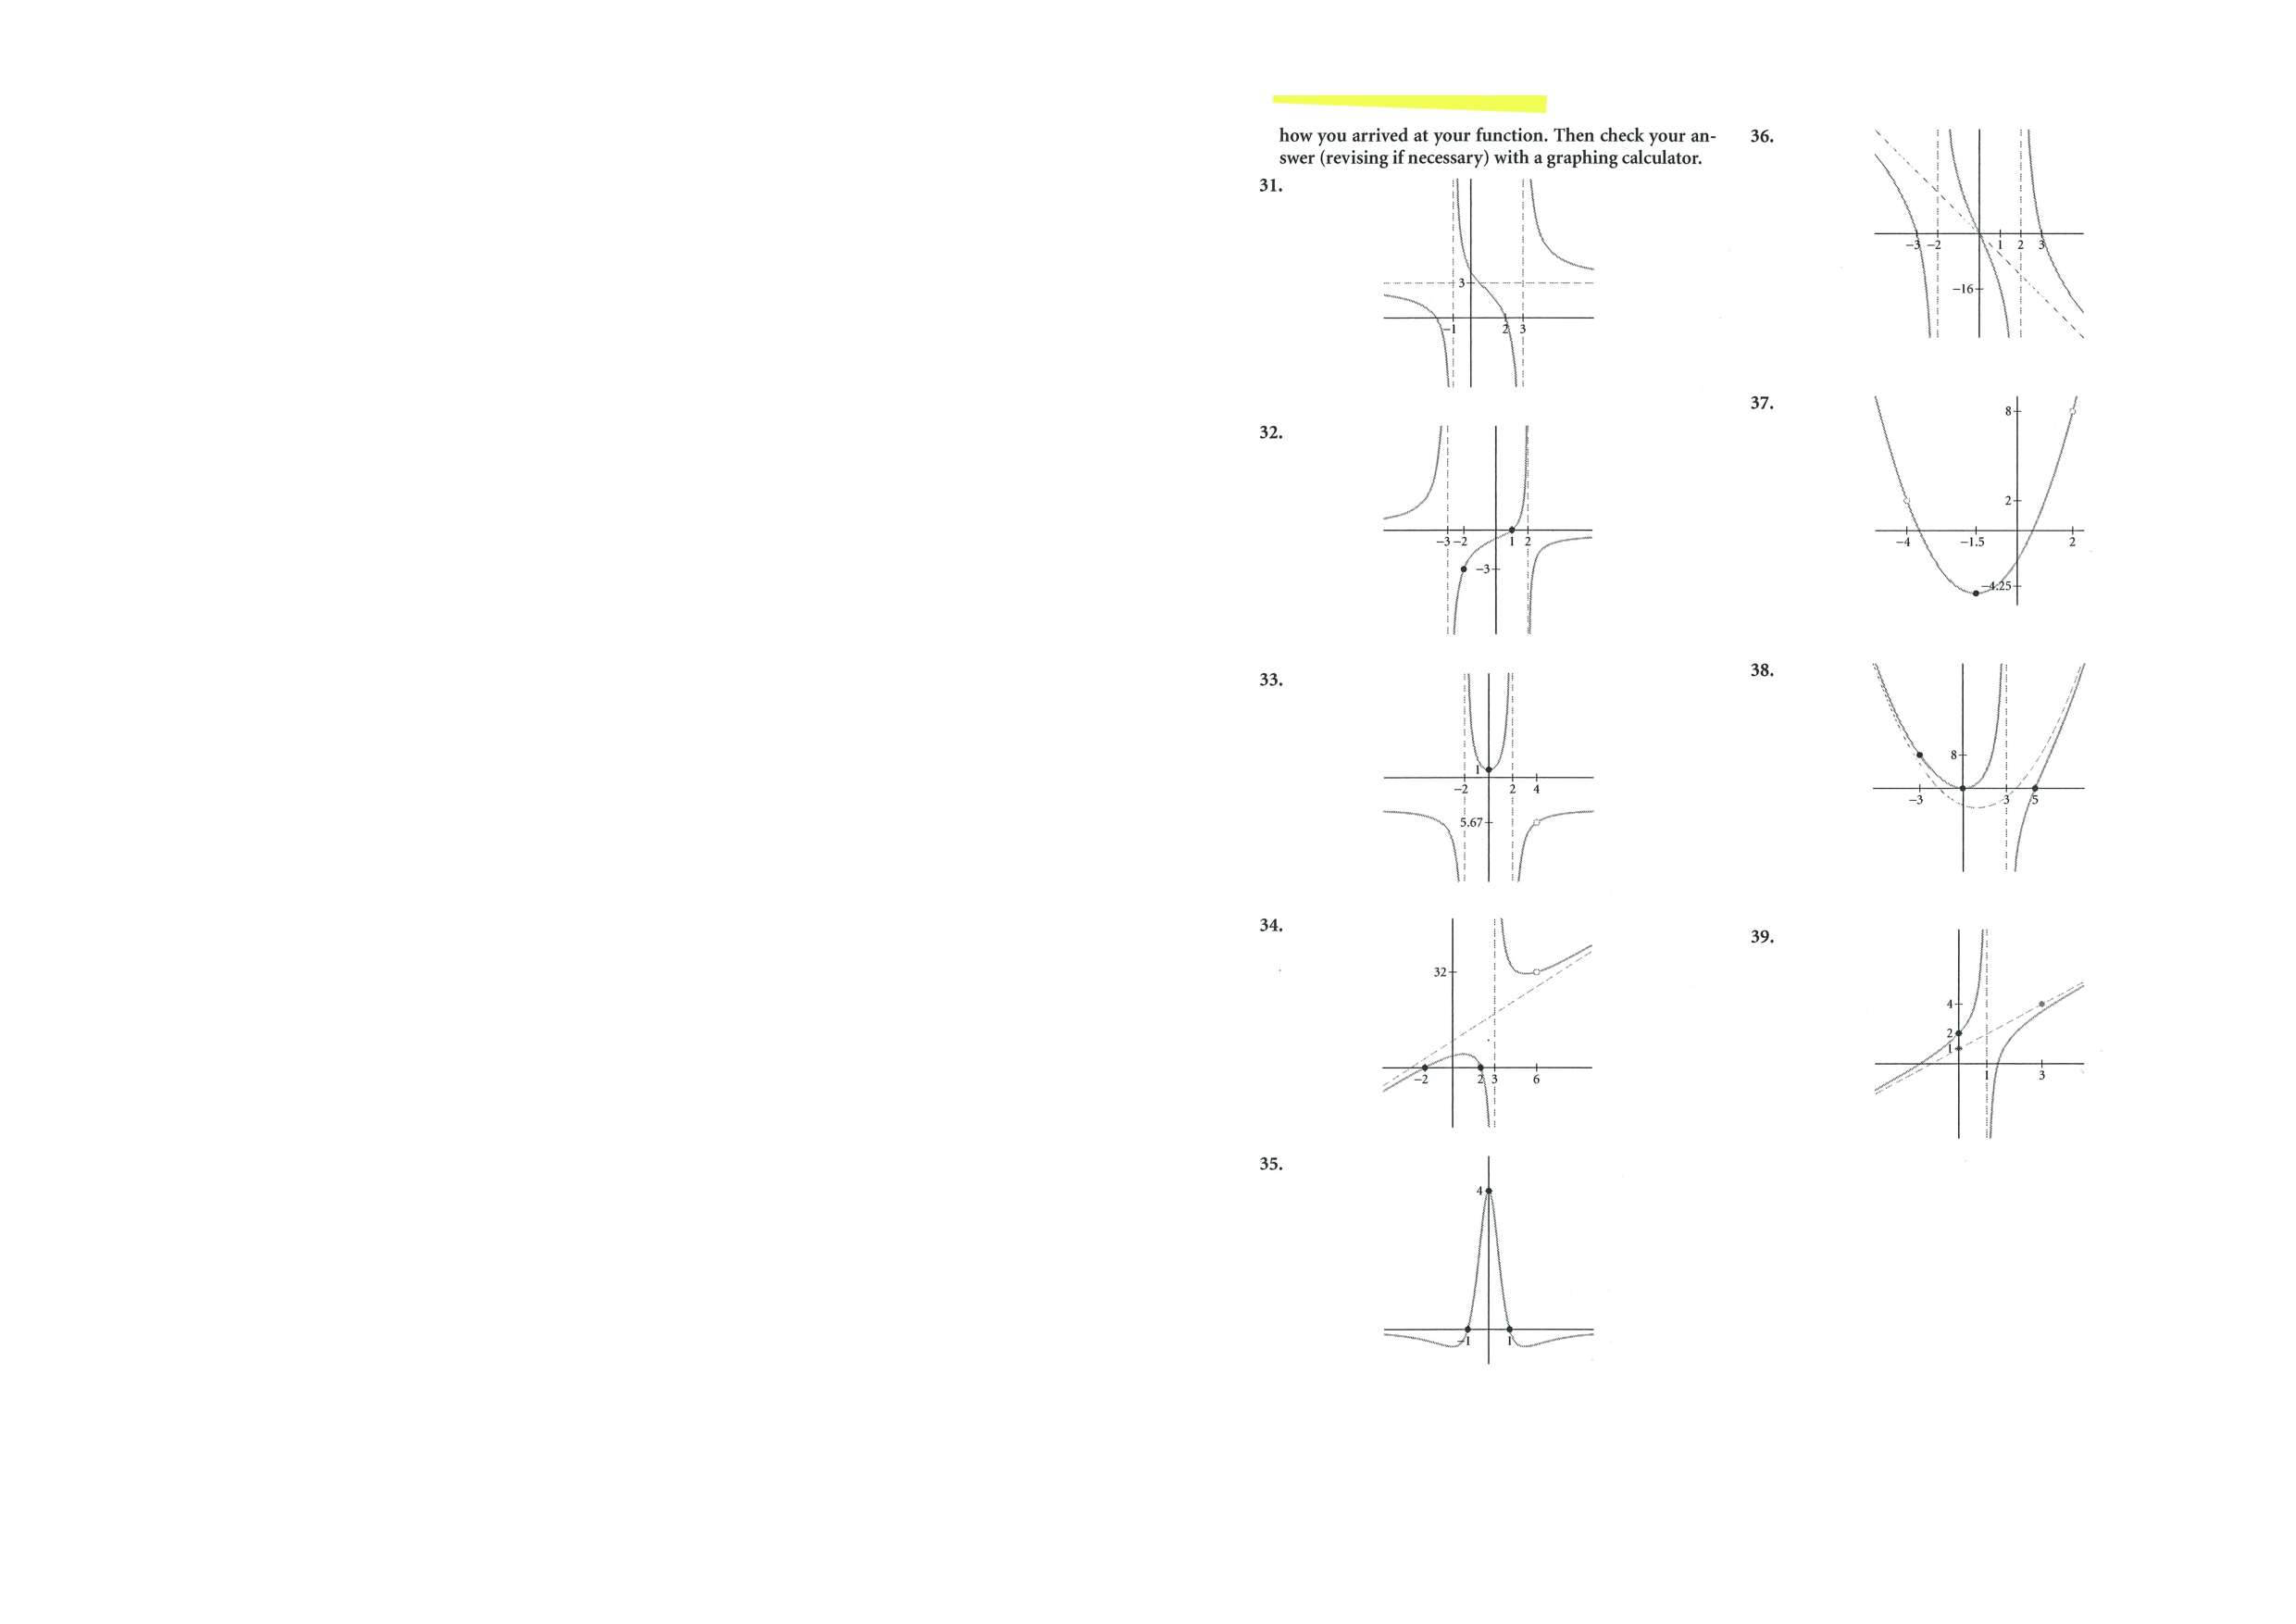
\includegraphics[width=\paperwidth]{\chapdir/0604xD.pdf}}



%									6 - 5
\newpage
\section{Asymptotes}
\noindent\makebox[\textwidth]{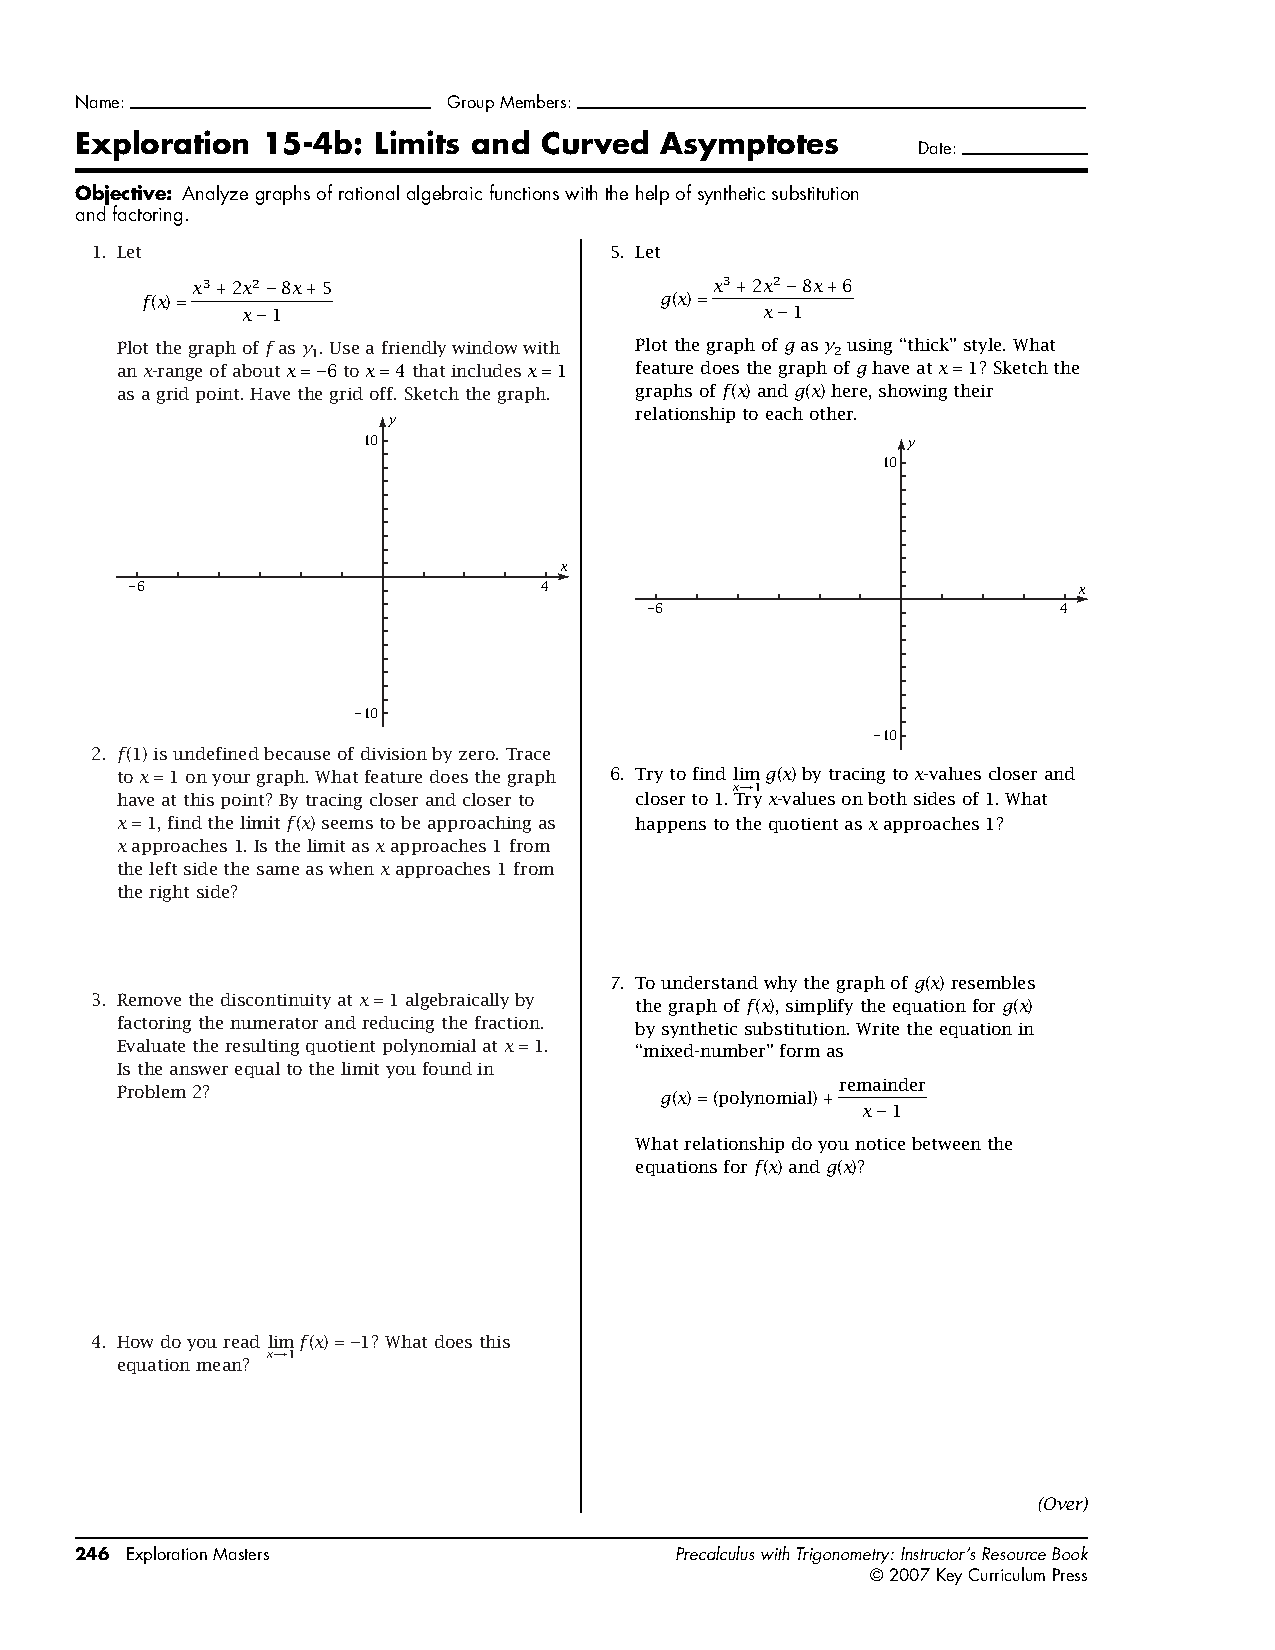
\includegraphics[width=\paperwidth]{\chapdir/0605p.pdf}}
%!TEX root =  ../main.tex

\objective{Compose and cecompose sums of power functions}

\subsection{Curvilinear Asymptotes}
We said last section that a rational function where the degree of the numerator is greater than
the degree of the denominator will have an asymptote defined by the quotient of the two,
ignoring the remainder.  Let us see an example.

$$
f(x)=\frac{(x+1)(x-2)(x-5)(x+5)}{(x-1)(x+2)}
$$

We can see that the first and last terms of the top will be $x^4 \dots +50$.  The bottom 
multiplies out to$x^2+x-2$.  The first two and the last two pairs in the numerator are easy 
to multiply: $(x^2-x-2)(x^2-25)$.  While a bit tortuous, multiply two trinomials is certainly
the easiest way to find the numerator, and it is $x^4-x^3-27x^2+25x+50$.  We can now find
the curvilinear asymptote.

\polylongdiv{x^4-x^3-27x^2+25x+50}{x^2+x-2}

The asymptote is a parabola!  It opens upward, has a $y$-intercept of -23 and a centerline 
at $x=1$.

\begin{figure}
\begin{centering}
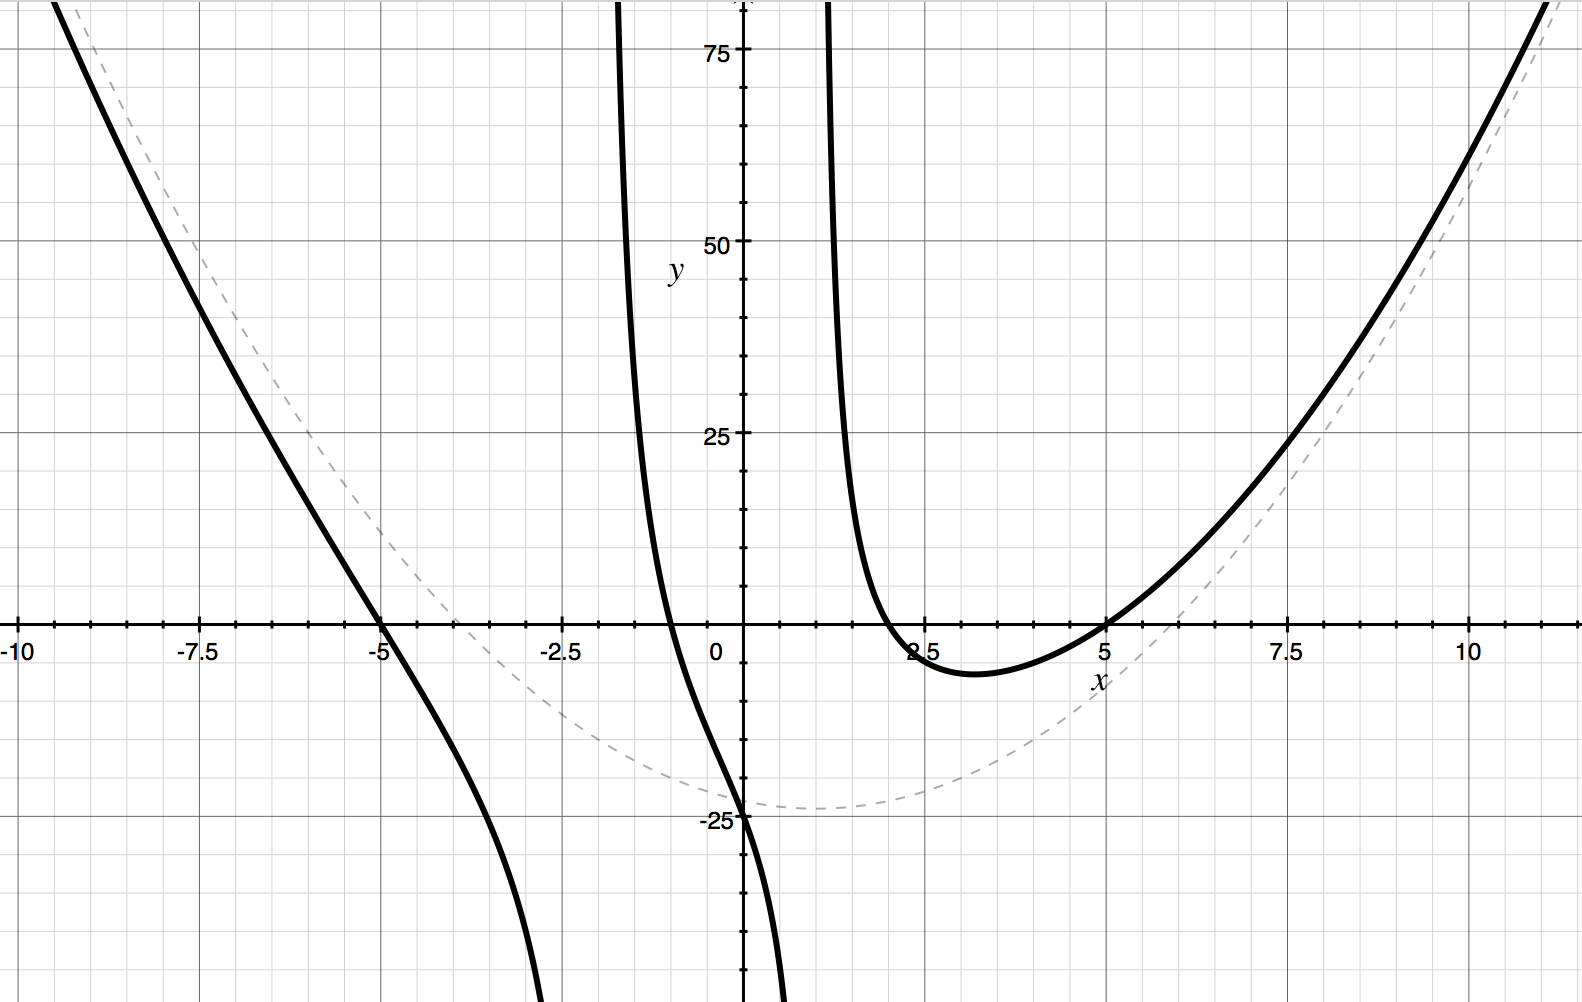
\includegraphics[width=\textwidth]{\chapdir/pics/curvilinear}
\caption{A function with a parabolic asymptote}
\end{centering}
\end{figure}

\subsection{Partial Fraction Decomposition}
Calculus is not concerned what the function does everywhere: we have the function itself
for that.  Calculus is satisfied local behavior, what a function does nearer and near to
certain places.  The curved asymptote we just found is more and more right, the larger 
(positive or negative) a number we plug into it.  We know how to find lines that behave
live the function almost any other point on the graph: tangent lines with a slope from
the derivative.  For example, at (5,0), the behavior can be modeled with 
$y-0 = \frac{47}{5}(x-5)$.  But what about around the asymptotes, at 1 and -2?  That is
where we bring back the ``remainder'' from the polynomial long division.

$\frac{44x+4}{x^2+x-2}$ is the non-asymptote part of the quotient, which we know is 
composed of $(x-1)(x+2)$ in the denominator.  Is there some way to rip it apart, into
two fractions, one with a denominator of (x-1) and another with (x+2)?  Let us suppose
there is, and that each fraction has a simple constant in the numerator.  That would
mean we are hypothesizing

$$
\frac{A}{x-1} + \frac{B}{x+2} = \frac{44x+4}{x^2+x-2}
$$

where $A$ and $B$ are plain numbers.  We can begin to figure out what they are by
``clearing the fraction'', multiplying by $x^2+x-2$ on both sides.  By factoring and canceling,
we get

$$
A(x+2) + B(x-1) = 44x + 4
$$

If we distribute and group for like terms, we get

$$
(A+B)x + (2A-B) = 44x + 4
$$

Now we already said $A$ and $B$ are numbers, so if we have $A+B x$'s on the left,
then $A+B$ must equal 44, and $2A-B$ must equal 4.  We can either add these two 
equations, or use a matrix and find that $A=16$ and $B=28$.  This means $\frac{16}{x-1}
+ \frac{28}{x+2} = \frac{44x+4}{x^2+x-2}$.

Additionally, we have decomposed the fraction into its partial fraction components,
a fancy way of saying we made it easy to integrate.  This assume that you know that
$\int \frac{1}{x} = \ln{|x|}$, which we will not prove until chapter 8.

In the vicinity of $x=1$, $\frac{16}{x-1}$ is a good model, and in the vicinity of $x=-2$,
$\frac{28}{x-2}$ is a good model of $f(x)$.


\subsection{Sums of Power Functions}
Finally, everything we have learned up until this point is also good for sums of 
power function that do not obey the definition of polynomials and rational functions.
For example, suppose you wanted to make a doorway modeled by the equation
$h(x) = \sqrt[3]{(x+4)^2}+\sqrt[3]{(x-4)^2}$ from -4 to 4.  If you had to program a 
machine lathe to make the curved top, what would its slope be at every point
on the interval?

We will need both the integral and the derivative of the function, but fortunately
it is the Power Rule all around.  $h'(x) = \frac{2}{3\sqrt[3]{x+4}}+\frac{2}{3\sqrt[3]{x-4}}$
and $H(x) = \frac{3}{5}\sqrt[3]{(x+4)^5}+\frac{3}{5}\sqrt[3]{(x-4)^5}+C$

~\vfill
\newpage
\subsection{Exercises}
two parts, in Kuta



\newpage
\section{Review}
\subsection{Chapter Review}
\subsection{Chapter Test}


